% Chapter 1

\chapter{The DEBORA Database} % Chapter title
\label{chap:debora}

\minitoc

\section{Introduction}

\label{ch:debora} % For referencing the chapter elsewhere, use \autoref{ch:introduction} 

The validation of any existing modeling of multiphase flows must rely on extensive databases from experimental investigations in operating conditions that are representative of industrial configurations in PWR. This naturally lead to an important demand for measurements of local phase-related properties of vertical pressurized subcooled boiling flows. 

\npar
To meet this need, CEA and EDF built a test facility called DEBORA in the 1990's. Its goal was to establish a consistent database of local measurements of the flow structure for vertical subcooled boiling freon Refrigerant 12 (R12) from the Onset of Nucleate Boiling to the Boiling Crisis.

\npar

In this chapter, we will describe the test section and analyze the available results from past measurements campaigns.


\section{Simulating PWR water using R12}

The choice of using R12 as the working fluid in the DEBORA loop emerged from the interesting properties that boiling freon presents when compared to the highly pressurized water in PWR cores. Indeed, the conditions for which the Boiling Crisis must be studied for water in PWR are:

\begin{itemize}
\item Pressure $P$ between 100 and 180 bar ;
\item Inlet liquid mass flux $G$ between 1000 and 5000~$\debm$ ;
\item Wall heat flux $\phi_{w}$ between 0.5 and 6 MW/m\up{2} ;
\item Inlet thermodynamic flow quality $x_{eq,in}$ between -0.4 and 0.4.
\end{itemize}

In those ranges, sensors dedicated to local measurements are not suited to sustain such conditions. 

\npar

The experimental strategy is then to "simulate" the aimed industrial conditions using a different fluid. It has to present thermophysical properties that allow to reproduce non-dimensional numbers of the industrial flow using less constraining operating conditions.

\npar

This explains the choice of R12 as it permits to transpose relevant parameters for PWR as detailed below.

\subsection{Conservation of the Phase Density Ratio}


Freon 12 can reach the same density ratio as water in PWR using limited pressurized conditions no larger than 30 bars. It is an important parameter to mimic the behavior of the boiling two-phase flow since it has a strong influence over the bubble size for example \cite{kocamustafaogullari_pressure_1983}.

\begin{equation}
\parth{\frac{\rho_{V,sat}}{\rho_{L,sat}}}_{P_{1}}^{water} = \parth{\frac{\rho_{V,sat}}{\rho_{L,sat}}}_{P_{2}}^{R12}
\end{equation} 
with $P_{2} < P_{1}$.

\npar

The evolution of the density ratio of water and R12 with pressure are shown on Figure \ref{fig:rhost_R12_PWR}.

\begin{figure}[!h]
\centering
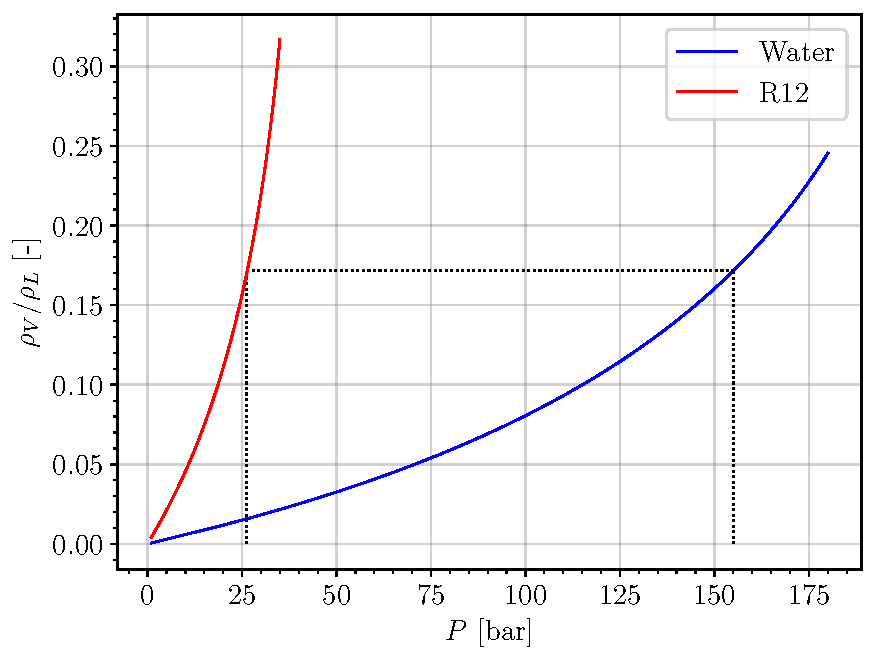
\includegraphics[width=0.6\linewidth]{img/DEBORA/rhost_R12_PWR.pdf}
\caption{Density ratio of pressurized R12 and water}
\label{fig:rhost_R12_PWR}
\end{figure}


For instance, we can see that R12 at approximatively 26 bar ($T_{sat} \approx 86.8 \degC$) has the same density ratio as water at 155 bar ($T_{sat} \approx 344.8 \degC$).

\npar

\begin{note*}{}
This tranposition criteria thus scales the operating pressure $P$ of the experiment.
\end{note*}

\subsection{Conservation of the Weber Number}

The Weber number is also similar to those encountered in PWR.

\begin{equation}
\We = \dfrac{G^{2}R}{\rho_{L} \sigma}
\end{equation}

This number characterizes physical phenomena such as bubble break-up or deformation under the influence of the liquid inertia.

\begin{figure}[!h]
\centering
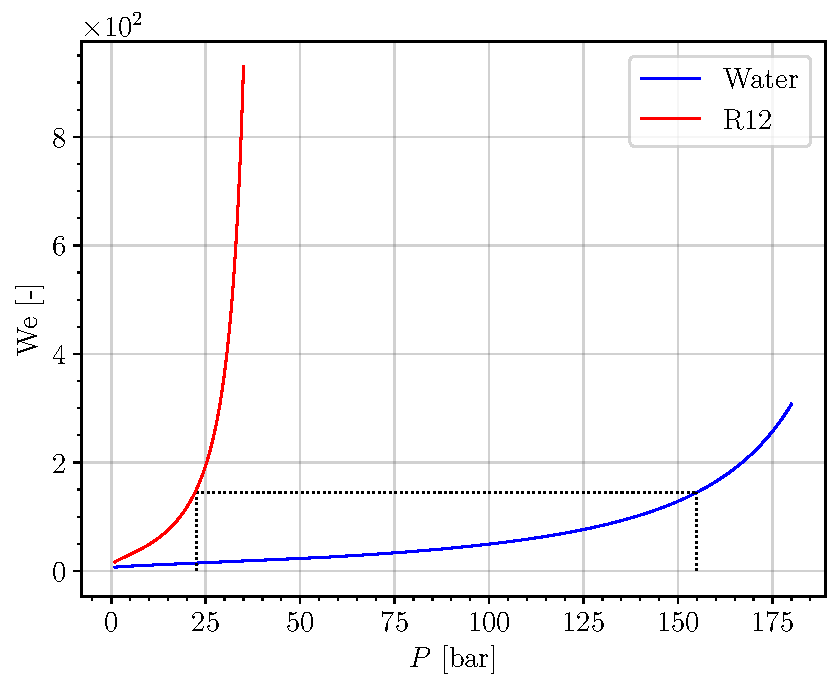
\includegraphics[width=0.6\linewidth]{img/DEBORA/We_R12_PWR.pdf}
\caption{Weber number for R12 and water at $G=2000~\debm$ and $R=0.1\mm$}
\label{fig:We_R12_PWR}
\end{figure}

Similar to the phase density ratio, Figure \ref{fig:We_R12_PWR} shows that Weber number equivalent to water at 155 bar can be reached with  R12 around 23 bar.

\npar

\begin{note*}{}
For a same value of $R$, this transposition scales the inlet liquid mass flux $G$.
\end{note*}

\subsection{Conservation of the Boiling Number}

The boiling number is defined as:

\begin{equation}
\Bo = \frac{\phi_{w}}{G h_{LV}}
\end{equation}  

It represents the comparison between the vapor mass flux $\phi_{w}/h_{LV}$ if all the heat flux contributes to phase change versus the inlet liquid mass flux. Thus, its value can be associated to the boiling and two-phase flow regime.

\begin{figure}[!h]
\centering
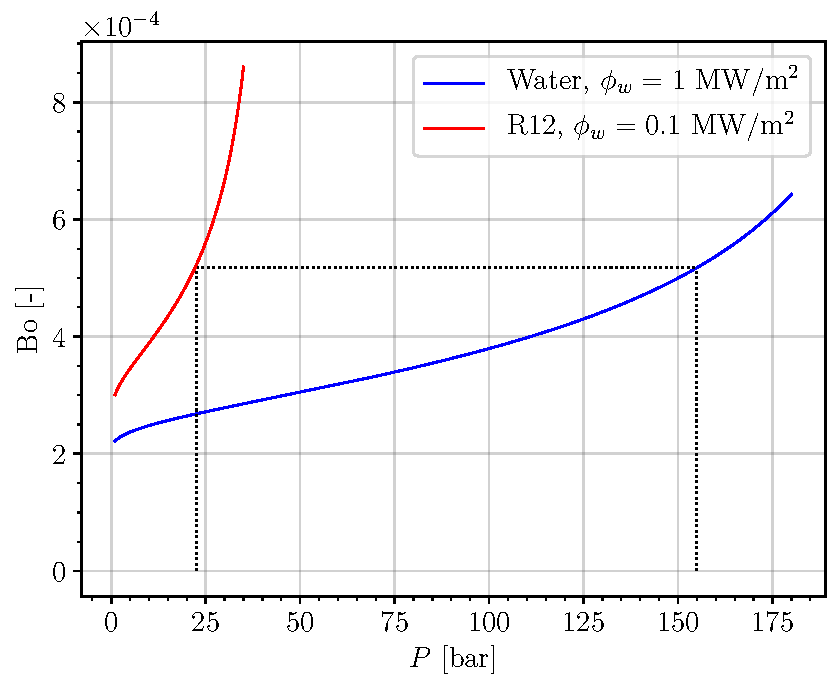
\includegraphics[width=0.6\linewidth]{img/DEBORA/Bo_R12_PWR.pdf}
\caption{Boiling number for R12 and water at $G = 2000~\debm$}
\label{fig:Bo_R12_PWR}
\end{figure}

Figure \ref{fig:Bo_R12_PWR} shows that Boiling number values similar to PWR can be reproduced using R12 with wall heat fluxes one order of magnitude lower and pressure around 23 bar.


\begin{note*}{}
This transposition criteria scales the applied heat flux $\phi_{w}$.
\end{note*}

\subsection{Conservation of the Inlet Thermodynamic Quality}

Water in PWR being highly subcooled to avoid boiling, reproducing the inlet subcooling in the DEBORA experiment allows to mimic the early stages of boiling between the ONB and OSV. It allows to reproduce Boiling Crisis by Departure from Nucleate Boiling for low quality flows. This is achieved through the inlet thermodynamic quality:


\begin{equation}
x_{eq,in} = \frac{h_{L,in} - h_{L,sat}}{h_{LV}}
\end{equation}

\begin{note*}{}
This transposition is achieved by scaling the R12 inlet temperature.
\end{note*}

\subsection{Same Geometry}

The last similarity achieved in the DEBORA experiment is related to the geometry. The heated length $L_{ch}$ of the test section is similar to the height of a nuclear fuel assembly and the hydraulic diameter $D_{h}$ is equal to that of a subchannel.


\subsection{Transposition ranges}

As a result of those conservation criteria, Table \ref{tab:R12_PWR_transposition} sums up the transposition ranges for each parameters.



\begin{table}[!h]
\centering
\begin{tabular}{c||c|c} 

Fluid & Water & Freon R12 \\
\hline \hline
$P$ [bar] & 100 - 180 & 14 - 30\\
%
$G$ [$\debm$] & 1000 - 5000 & 1000 - 5000\\
%
$\phi_{w}$ [MW/m$^{2}$] & 0.5 - 6 & 0.05 - 0.65\\ 
%
$x_{eq,in}$ [-] & (-0.4) - (+0.4) & (-0.4) - (+0.4)\\
\hline
\hline 
${\rho_{V,sat}}/{\rho_{L,sat}}$ [-] & 0.08 - 0.25 & 0.07 - 0.22\\
%
$\We$ [-] & 49.5 - 307.1 & 69.1 - 365.8\\
%
$\Bo \times 10^{-3} $ [-] &  $0.19$ - $3.86$ & $0.21$ - $4.33$ \\
\hline
\end{tabular}

\caption{Water R12 scaling, $R=0.01$mm for $\We$}
\label{tab:R12_PWR_transposition}

\end{table}



\section{Description of the Test Section}

\subsection{Geometrical Description}
To apply the aforementioned transport criteria, four thermal-hydraulic control parameters are imposed in the test section:

\begin{itemize}
\item The outlet pressure $P$ ;
\item The inlet mass flow rate $G \times S_{in}$ with $S_{in} = \pi R^{2} \approx 2.9 \times 10^{-4}$ m\up{2} the inlet area ;
\item The inlet liquid temperature $T_{L,in}$ ;
\item The electrical power transferred to the liquid $\phi_{w}\times S_{heat}$ with $S_{heat}$ the heated area. 
\end{itemize}

\begin{figure}[!h]
\centering
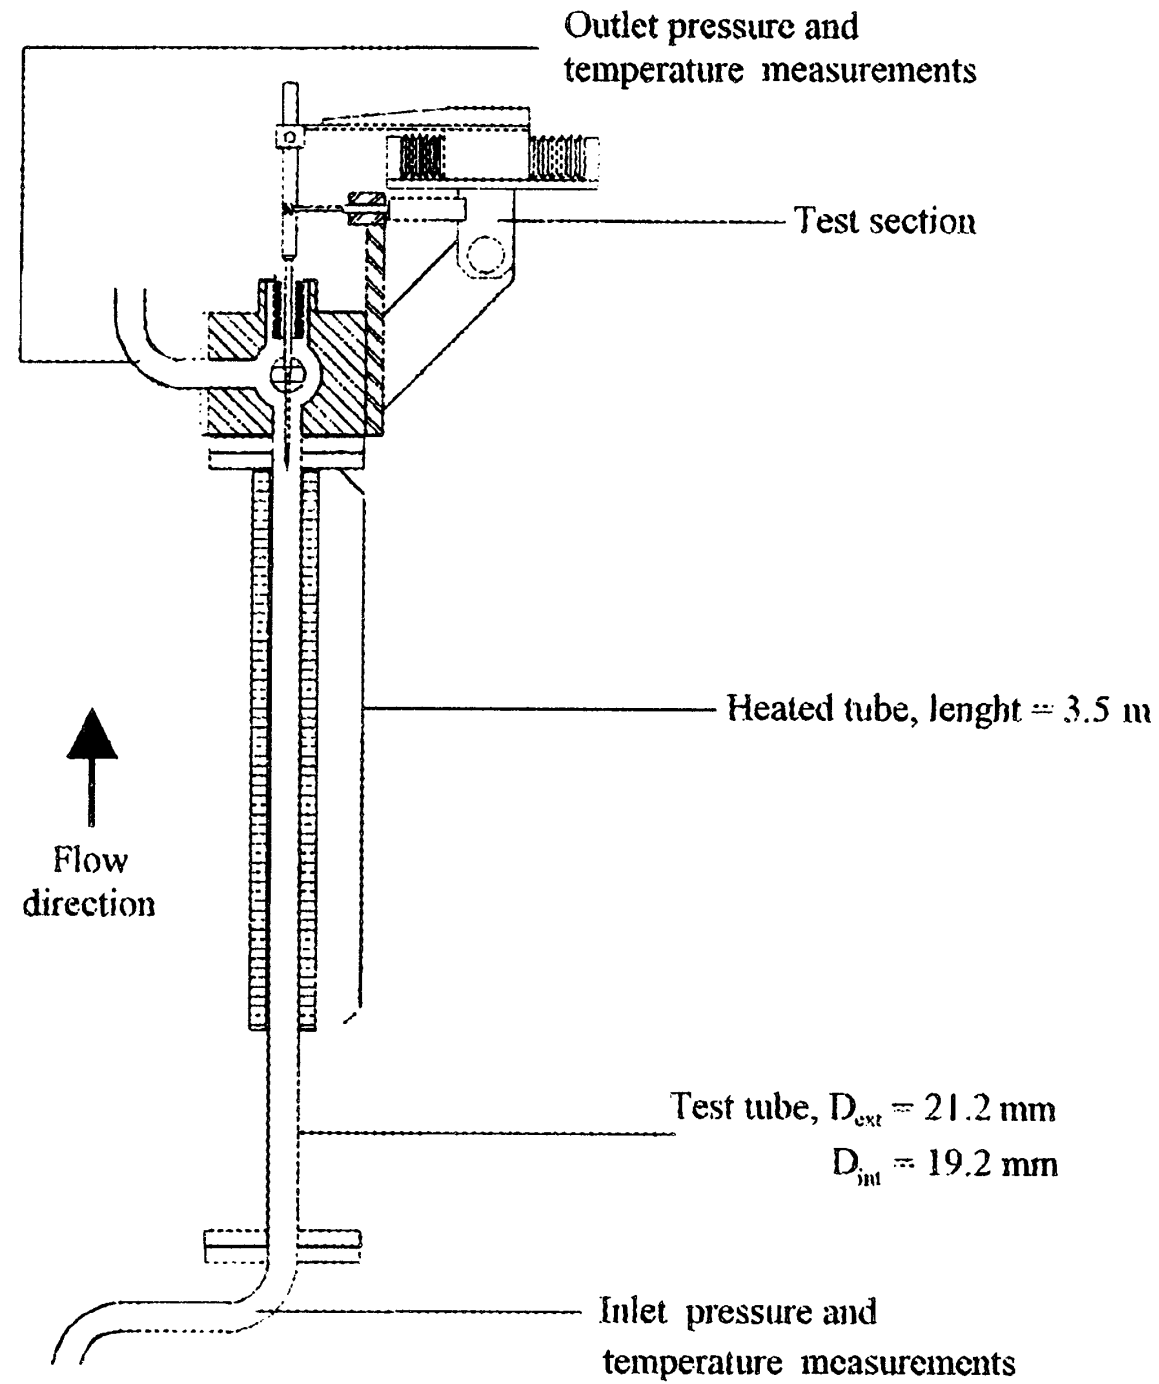
\includegraphics[width=0.7\linewidth]{img/DEBORA/debora_sketch.png}
\caption{Sketch of the DEBORA test section. Adapted from \cite{garnier_local_2001}.}
\label{fig:sketch_debora}
\end{figure}


The test section in presented on Figure \ref{fig:sketch_debora}. It consists of an inconel tube with inner diameter $D_{h}=19.2$ mm, a 1 mm thickness and a heated length $L_{heat}$=3.5 m. A detailed description of the whole experimental loop is given in Garnier \etal \cite{garnier_local_2001}.

\subsection{Measurement Instrumentation}

The control parameters are adjusted and measured using pressure, temperature, flow rate and power measurements. They are further detailed in Cubizolles \cite{cubizolles_etude_1996}.

\npar

The local measurements are conducted at the end of the heating length using a controllable probe that can cover the whole diameter of the test section with an accuracy of $10 \mu$m . Only one diameter is covered since the chosen geometry induces an axisymmetry.

Three type of measurements have been conducted over different experimental campaigns.

\subsubsection{Mono-Optical Probe Measurements}


Optical probe measurement rely on the difference of optical refractive index between the liquid and vapor phase. Using an optical fiber in which light is emitted towards the probe tip allows to detect the actual phase flowing on the probe. 

\npar

The resulting signal is called a Phase Indicator Function (PIF) which looks like to a square signal (Figure \ref{fig:FIP}) that can be post-processed to identify the average time spent by the probe in each phase and then estimate their volume fraction \eg the void fraction. 


\begin{figure}[!h]
\centering
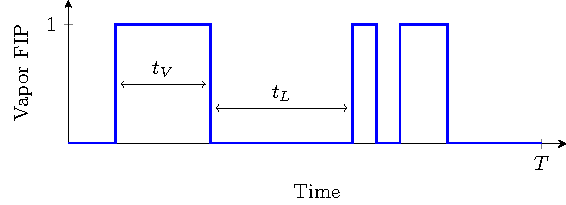
\includegraphics[width=0.65\linewidth]{img/DEBORA/FIP.pdf}
\caption{Example of Phase Indicator Function signal}
\label{fig:FIP}
\end{figure}



If the PIF is measured over a period $T$, the void fraction $\alpha$ at the measurement point $x$ can be estimated by:


\begin{equation}
\alpha\parth{x}\ = \nu\parth{x} \overline{t_{V}} = \frac{1}{T} \sum t_{V}
\end{equation}
where $\nu$ is called the interference frequency that represents the number of phase interface detection per second by the probe.

\begin{note*}{}
This measurement technique was performed in the \textbf{measurement campaign C2900} where void fraction profiles at the outlet were obtained for various flow conditions.
\end{note*}

\subsubsection{Bi-Optical Probe Measurements}


Using the technology of the optical phase dectection, adding a second optical probe permits to measure more parameters of the two-phase flow. Indeed, the use of two probes placed close to each other with a small shift in the flow direction (Figure \ref{fig:optical_probe}) allows to estimate the velocity of the interface between the two probes by measuring the time difference between the two PIF.


\begin{figure}[!h]
\centering
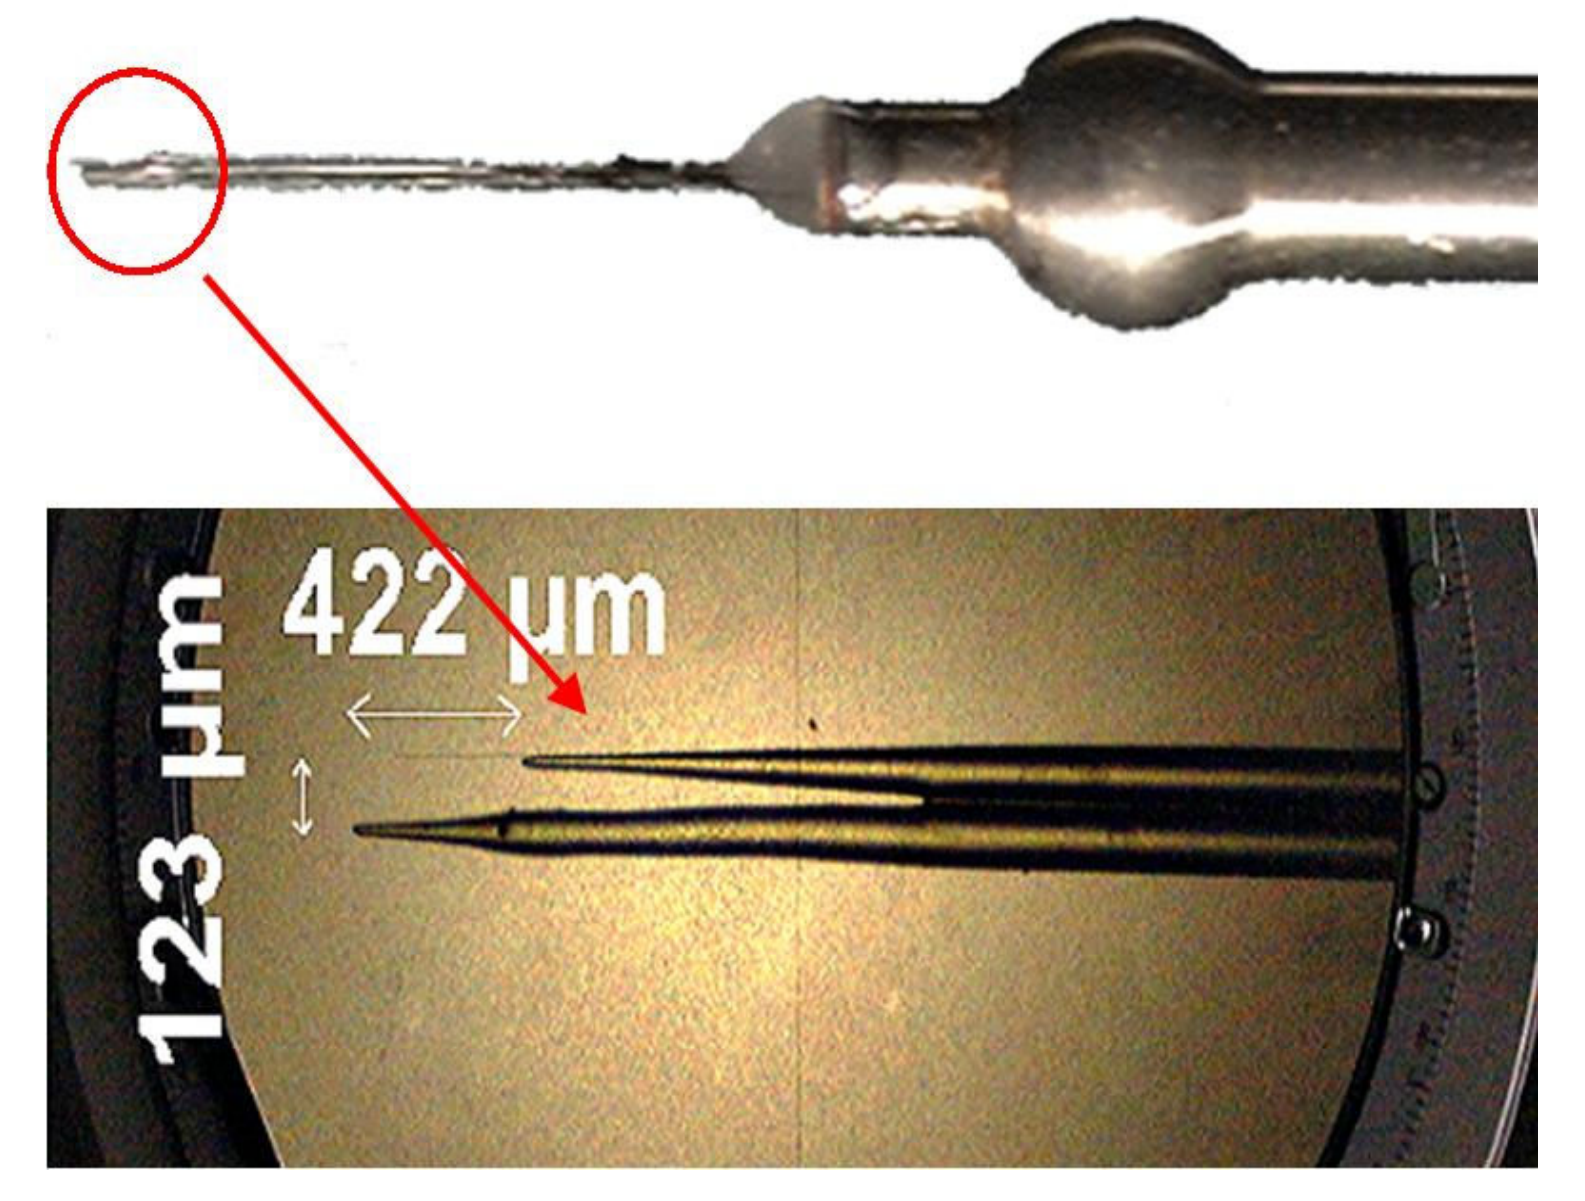
\includegraphics[width=0.65\linewidth]{img/DEBORA/optical_probe.png}
\caption{Picture of the bi-optical probe with a zoom over the two optical fibers. Reproduced from \cite{gueguen_contribution_2013}.}
\label{fig:optical_probe}
\end{figure}

\npar

Considering the following assumptions:

\begin{itemize}
\item The flow is mainly one-directional in aligned with the probes ;
\item The vapor phase is composed of spherical inclusions ;
\item The velocity gradient and center density gradient are small along a bubble diameter length.
\end{itemize}

Then we can estimate: 

\begin{itemize}
\item The vapor axial velocity $U_{V,z}$ that can be supposed equal to the measured interface velocity between the probes ;
\item The interfacial area density $a_{i}$:
\begin{equation}
a_{i} = \frac{4 \nu }{U_{V,z}}
\end{equation}
\item The bubble Sauter diameter:
\begin{equation}
D_{V} = \frac{6 \alpha }{a_{i}}
\end{equation}
\end{itemize}


\begin{note*}{}
This measurement technique was performed in the \textbf{measurement campaign C3000}.
\end{note*}


\subsubsection{Thermocouples Measurements}

Thermal measurements are conducted using chromel-alumel thermocouples. The liquid temperature is measured along the outlet diameter at the end of the heating length. Wall temperature measurements are conducted with 4 thermocouples placed at different heights (1.465 m, 2.465 m, 2.965 m, 3.485 m) on the outside of the tube.

\begin{note*}{}
This measurement technique was performed in the \textbf{measurement campaign C800}.
\end{note*}



\section{Measurements Campaigns and Results}

\subsection{Cases Nomenclature and Test Series}

As mentioned before, three different campaigns have been performed:

\begin{itemize}
\item Campaign C2900 with solely void fraction measurements using mono-optical probe ;

\item Campaign C3000 with void fraction, vapor velocity, bubble Sauter diameter and interfacial area density measurements using bi-optical probe ;

\item Campaign C800 with liquid and wall temperature measurements using thermocouples.
\end{itemize}


Each measurement series is conducted under fixed outlet pressure, liquid mass flux and electrical power. Inlet temperature is then changed to cover different inlet quality. Experimental cases are named in the form C\textbf{cc}G\textbf{g}P\textbf{pp}W\textbf{ww}Te\textbf{tt} with \textbf{cc} the campaign number (29, 30 or 8), \textbf{g} the inlet mass velocity ($G$ in t/m\up{2}/s), \textbf{pp} the outlet pressure ($P$ in bars), \textbf{ww} the total heat power applied ($\Phi_{w}$ in kW) and \textbf{tt} the inlet temperature ($T_{L,in}$ in K). For instance, the case named C30G2P26W16Te66 has been conducted with $P=26.2$ bar, $G=2049\ \debm$, $\Phi_{w}=15.6$ kW $\equiv$ $\phi_{w} =73.89$ kW/m\up{2} and $T_{L,in} = 66.59 \degC$.


\begin{table}[!h]
\scriptsize
\centering


\noindent\makebox[\textwidth]{
\renewcommand{\arraystretch}{2.0}
\begin{tabular}{|c|c|c|c|c|c|c|c|c|c|c|c|c|c|c|c|c|c|c|}
\hline
P                   & G & W16 & W17 & W23 & W24 & W25 & W27 & W29 & W30 & W31 & W33 & W34 & W36 & W38 & W39 & W40 & W42 & W44 \\
\hline
\hline
\multirow{3}{*}{14} & 2 &  $\bigcirc$ $\bigtriangledown$ $\bigtriangleup$  & $\bigtriangleup$    &     &    &     &     &     &     &     &     &     &     &     &     &     &     &     \\
                    & 4  &     &     &     &  $\bigcirc$   &     &     &     &     &     &     &     &     &     &     &     &     &     \\
                    & 5  &     &     &     &     &     &     & $\bigtriangledown$    &  $\bigtriangledown$   &     &  $\bigtriangledown$   &  $\bigtriangledown$   &  $\bigtriangledown$   &   $\bigtriangledown$  &    & $\bigtriangledown$   &  $\bigtriangledown$   &     \\
                    \hline
\multirow{3}{*}{26} & 2  &  $\bigcirc$ $\bigtriangledown$ $\bigtriangleup$  &     &     &     &     &     &     &     &     &     &     &     &     &     &     &     &     \\
                    & 3 &     &     &  $\bigtriangledown$ $\bigtriangleup$  &     &  $\bigtriangledown$   &  $\bigtriangledown$ $\bigtriangleup$   &   $\bigtriangledown$  &     & $\bigtriangledown$  $\bigtriangleup$   &  $\bigtriangledown$   &     &  $\bigtriangledown$   $\bigtriangleup$ &  $\bigtriangledown$   &  $\bigtriangledown$   & $\bigtriangledown$ $\bigtriangleup$   & $\bigtriangledown$    &  $\bigtriangledown$ $\bigtriangleup$   \\
                    & 5  & $\bigcirc$   &     &     &  $\bigcirc$   &     &     &     &     &     &     &     &     &     &     &     &     &     \\
\hline
\end{tabular}
}

\npar

\noindent\makebox[\textwidth]{
\renewcommand{\arraystretch}{2.0}
\begin{tabular}{|c|c|c|c|}
\hline
P                   & G & W12 & W14\\
\hline
\hline
30                  & 1 &  $\bigtriangledown$   &  $\bigtriangledown$   \\
\hline
\end{tabular}
}

\caption{Test matrix of the DEBORA cases. $\bigcirc$: C800 - $\bigtriangledown$: C2900 - $\bigtriangleup$: C3000 }%\newline \scriptsize{Written at Plateau d'Auguste, Hyper U, Saintes} }
\label{tab:debora_matrix}
\end{table}


If we want to obtain a full description of the two-phase flow from the DEBORA tests, we need to have measurements from campaigns C3000 and C800 (flow topology and thermal) with the same control parameters. Table \ref{tab:debora_matrix} unfortunately shows that only very few test series between C3000 and C800 have common operating conditions, namely:

\begin{itemize}
\item Series 8G2P14W16 and 30G2P14W16 ;
\item Series 8G2P26W16 and 30G2P26W16.
\end{itemize}

Other flow conditions have either been covered with thermal measurements or topology measurements but not both. 

\begin{remark*}{}
Cases from the campaign C2900 would only be relevant for void fraction profiles comparison. Estimations of the bubble diameter can not be achieved except if one assumes a velocity profile as suggested by Cubizolles \cite{cubizolles_etude_1996} and re-used by Guéguen \cite{gueguen_contribution_2013} who supposes:

\begin{equation}
U_{V,z}\parth{r} \approx U_{M,z}\parth{r} = 1.22 \frac{G}{\spavg{\rho_{M}}} \parth{ \frac{R-r}{R}}^{1/7}
\label{eq:ugz_C29}
\end{equation}
where $U_{M,z}$ is the mixture axial velocity, assuming a mechanical equilibrium between the phases.

\end{remark*}


For further studies, we will mainly focus on the G2P26W16 and G2P14W16 test series. Although we will mainly rely on the results from the C3000 campaign (where vapor velocity was actually measured) for flow topology qualification, we will evaluate the assumption of Eq. \ref{eq:ugz_C29} with the C2900 measurements.


\subsection{Verification of Control Parameters Coherency}

For each case, the total heat heat input $\Phi_{w}$ is given along with the inlet mass flux $G$, inlet liquid temperature $T_{L,in}$ and outlet quality $x_{eq,out}$. To verify the consistency of those values, we can recalculate the outlet quality:

\begin{equation}
x_{eq,out,calc} = \frac{h_{M,out,calc} - h_{L,sat}}{h_{LV}}
\label{eq:xeq_out}
\end{equation}
with $h_{M,out,calc}$ the recalculated outlet mixture enthalpy:

\begin{equation}
h_{M,out,calc} = h_{in} + \frac{\Phi_{w}}{G S_{in}} = h_{in} + \frac{4\phi_{w}L_{heat}}{G D_{h}}
\end{equation}
with $h_{in}$ the inlet enthalpy calculated from the fluid properties using the inlet liquid temperature.

\npar
The difference between the given and recalculated outlet quality can also be converted to input power error by recalculating the heat needed to reach the given $x_{eq,out}$:

\begin{equation}
\Phi_{w,calc} = \frac{G  \pi R^{2}}{\underbrace{\crocht{x_{eq,out}h_{LV}+h_{L,sat}}}_{h_{M,out}} - h_{L,in}}
\end{equation}

\npar 


Moreover, for a given set of experiments at the same $P$, $G$ and $\Phi_{w}$ changing the inlet quality can be associated to moving the measurement diameter along the axial direction following the relationship: 

\begin{equation}
x_{eq}\parth{z} = x_{eq,in} + \frac{4 \phi_{w} z }{G D_{h} h_{LV}}
\end{equation}

Thus, taking the maximum inlet quality case $x_{eq,in, max}$ as a reference ($z=3.5$ m), we can estimate the corresponding measurement height $z_{eq}$ of each other cases if the inlet quality was $x_{eq,in, max}$.

\npar

We calculated the equivalent heights and outlet quality / power input errors for two series of the C3000 campaigns. Results are displayed on Tables \ref{tab:30P14_recalc} and \ref{tab:30P26_recalc}.



\begin{table}[!h]
\centering
\begin{tabular}{c|c|c|c|c|c|c}
$T_{L,in}$ {[}K{]} & $x_{eq,in,calc}$ {[}-{]} & $x_{eq,out,calc}$ {[}-{]} & $x_{eq,out}$ {[}-{]} & $z_{eq}$ {[}m{]} & $x_{eq,out}$ error {[}-{]} & $\Phi_{w}$ error {[}kW{]} \\
\hline
\hline
22.39  &  -0.317  &  -0.0821  &  -0.0832  &  1.075  &  0.114 \% &  -0.078 \\
%
26.8  &  -0.28  &  -0.0422  &  -0.0431  &  1.653  &  0.089 \% &  -0.061\\
%
28.76  &  -0.263  &  -0.0267  &  -0.0273  &  1.896  &  0.056 \% &  -0.038\\
%
30.08  &  -0.252  &  -0.0152  &  -0.0157  &  2.065  &  0.05 \% &  -0.034\\
%
31.39  &  -0.241  &  -0.004  &  -0.0043  &  2.234  &  0.035 \% &  -0.023\\
%
38.95  &  -0.175  &  0.0674  &  0.0681  &  3.229  &  -0.072 \% &  0.049\\
%
39.96  &  -0.166  &  0.077  &  0.0776  &  3.357  &  -0.063 \% &  0.042\\
%
41.16  &  -0.155  &  0.0875  &  0.0882  &  3.509  &  -0.064 \% &  0.043
\end{tabular}
\caption{Recalculated control parameters for the 30G2P14W16 cases. ($T_{sat} = 58.07\degC$)}
\label{tab:xout_30P14_recalc}
\end{table}


\begin{table}[!h]
\centering
\begin{tabular}{c|c|c|c|c|c|c}
$T_{L,in}$ {[}K{]} & $x_{eq,in,calc}$ {[}-{]} & $x_{eq,out,calc}$ {[}-{]} & $x_{eq,out}$ {[}-{]} & $z_{eq}$ {[}m{]} & $x_{eq,out}$ error {[}-{]} & $\Phi_{w}$ error {[}kW{]} \\
\hline
\hline
58.57              & -0.395                   & -0.0893                   & -0.0819              & 1.792            & -0.747 \%                  & 0.381                     \\
60.54              & -0.370                   & -0.0650                   & -0.0578              & 2.072            & -0.722 \%                  & 0.369                     \\
62.54              & -0.344                   & -0.0392                   & -0.0318              & 2.369            & -0.741 \%                  & 0.378                     \\
64.6               & -0.318                   & -0.0123                   & -0.0050              & 2.674            & -0.736 \%                  & 0.376                     \\
66.59              & -0.292                   & 0.0140                    & 0.0213               & 2.973            & -0.728 \%                  & 0.371                     \\
68.57              & -0.266                   & 0.0402                    & 0.0473               & 3.271            & -0.716 \%                  & 0.365                     \\
70.59              & -0.239                   & 0.0670                    & 0.0743               & 3.583            & -0.723 \%                  & 0.369                    
\end{tabular}
\caption{Recalculated control parameters for the 30G2P26W16 cases. ($T_{sat} = 86.81\degC$)}
\label{tab:xout_30P26_recalc}
\end{table}

As we can see, the given values of outlet quality for the 30G2P14W16 tests are coherent with the one-dimensional enthalpy balance with errors mostly less than 0.1\% on the recalculated quality and less than 100 W on the recalculated power input. This naturally leads to an equivalent height very close to $3.5$ m for the hottest case.


However, a more significant error is observed on the 30G2P26W16 cases where errors up to 0.75\% on the outlet quality and close to 0.4 kW on the power input are found. Those values are significant especially for cases close to saturation where uncondensed vapor will start to appear in the bulk. Moreover, this results in an equivalent height 8.3 cm longer than the actually 3.5m heated length.

\npar

Since the inlet temperature, mass flux and power input are controlled parameters for each test, it is likely that the error may come from the given value of outlet quality $x_{eq,out}$ which is calculated and not imposed.

\begin{note*}{}
Similar quality / input power errors were obtained on corresponding C29 and C8 campaigns:

\begin{itemize}
\item Negligible errors on for 29G2P14W16 and 8G2P14W16 cases ;
\item Roughly 0.7 \% outlet quality error and 0.3 to 0.4 kW power error for 29G2P26W16 and 8G2P26W16 cases. 
\end{itemize}
\end{note*}

\subsection{Qualitative Analysis of the Experimental Results}

On Figures \ref{fig:30G2P26W16_exp}, \ref{fig:8G2P26W16_exp}, \ref{fig:30G2P14W16_exp} and \ref{fig:8G2P14W16_exp} we respectively plot the experimental measurements of cases 29/30G2P26W16, 8G2P26W16, 29/30G2P14W16 and 8G2P14W16. The colorbar representing the oulet quality of each test is based on the computed value of $x_{eq,out}$ (Eq. \ref{eq:xeq_out}).


\subsubsection{G2P26W16 cases}

\begin{figure}[h!]
\centering

\subfloat[Void fraction measurements]{
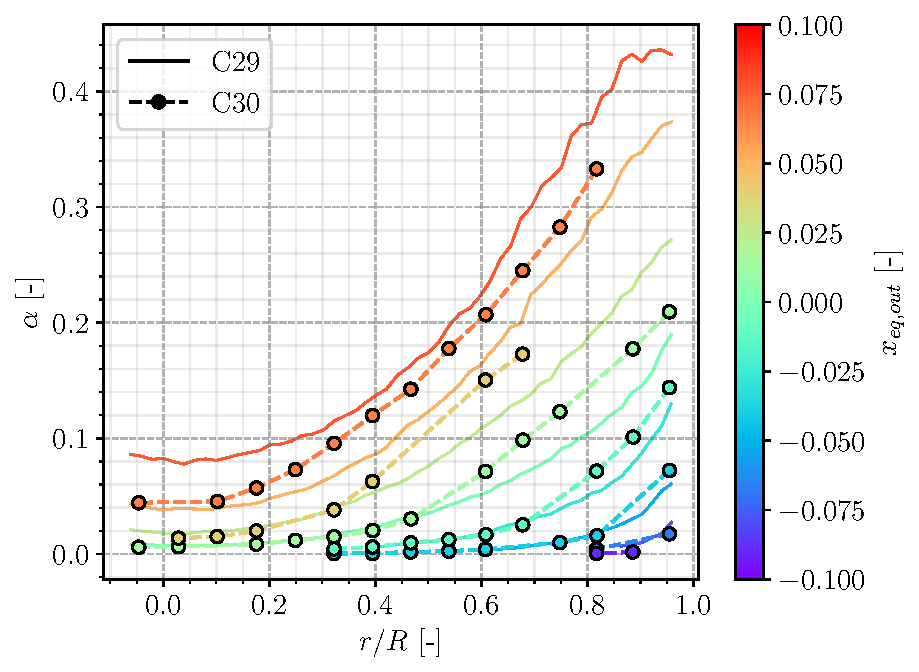
\includegraphics[width=0.5\linewidth]{img/DEBORA/30G2P26W16/30G2P26W16_alpha.pdf}
\label{fig:G2P26W16_alpha}
}
\subfloat[Vapor velocity measurements]{
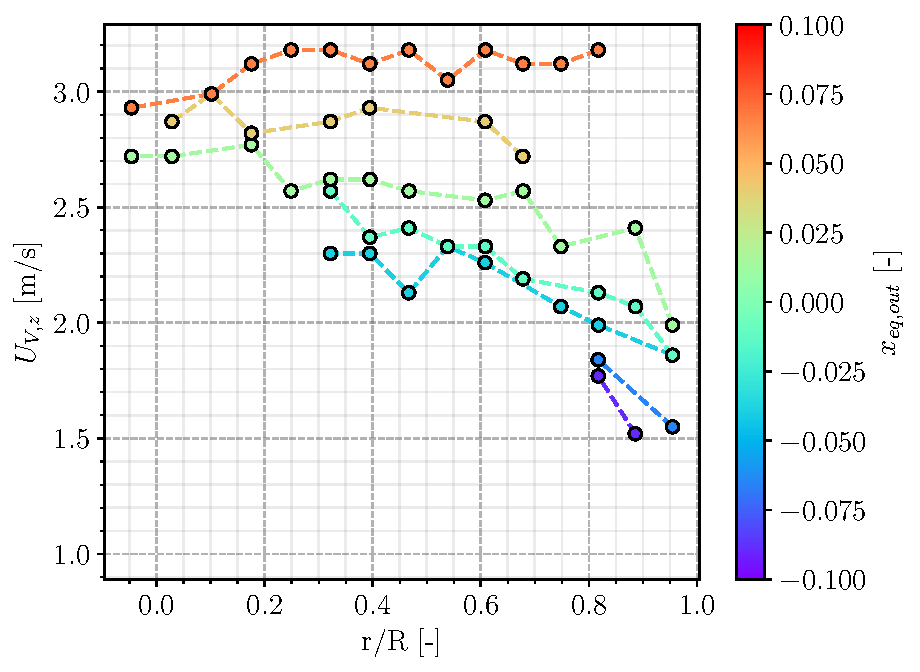
\includegraphics[width=0.5\linewidth]{img/DEBORA/30G2P26W16/30G2P26W16_ugz.pdf}
\label{fig:G2P26W16_ugz}
}
\\
\subfloat[Bubble diameter measurements]{
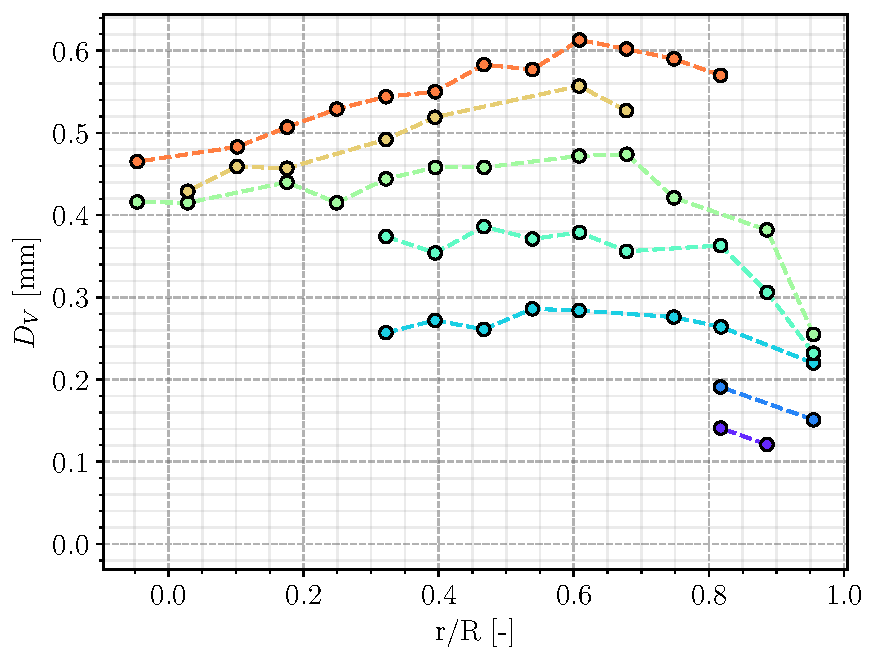
\includegraphics[width=0.5\linewidth]{img/DEBORA/30G2P26W16/30G2P26W16_dv.pdf}
\label{fig:G2P26W16_dv}
}
\subfloat[Interfacial area concentration measurements]{
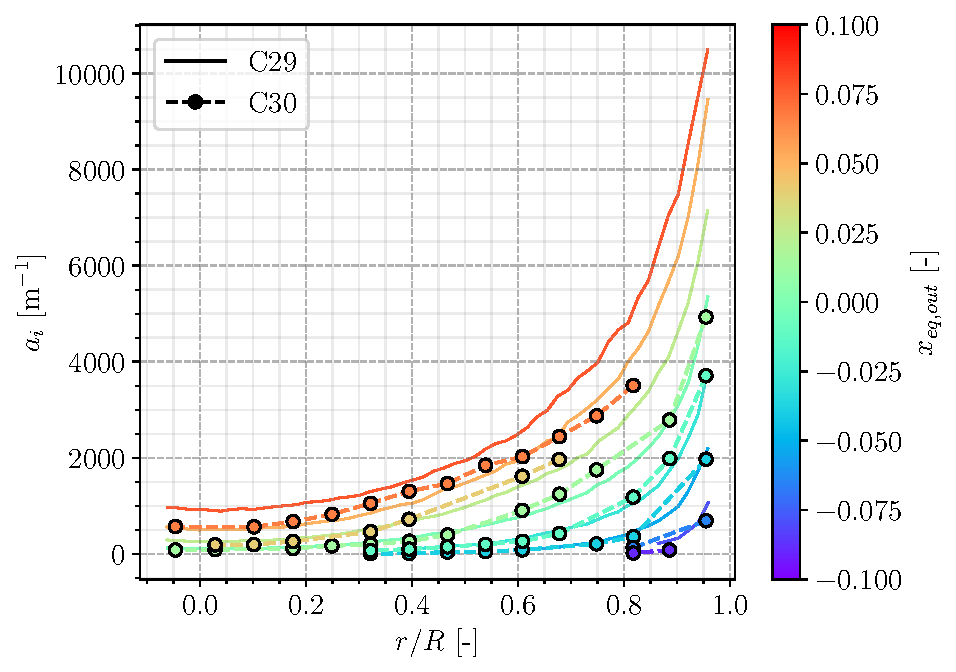
\includegraphics[width=0.5\linewidth]{img/DEBORA/30G2P26W16/30G2P26W16_ai.pdf}
\label{fig:G2P26W16_ai}
}


\caption{30G2P26W16 and 29G2P26W16 results}
\label{fig:30G2P26W16_exp}
\end{figure}

Void fraction profiles obtained in for C2900 (single optical probe) and C3000 (bi-optical probe) cases are compared to verify the consistency of the measurements (Figure \ref{fig:G2P26W16_alpha}). The two campaigns are in good agreement with each other, displaying a void fraction profile monotonously increasing with the outlet quality. The estimation of the vapor velocity by Eq. \ref{eq:ugz_C29} for the C29 results is acceptable but presents an growing underestimation as the outlet title increases (Figure \ref{fig:G2P26W16_ugz}). This results in bubble diameter underestimation close to the wall and consequently interfacial area overestimation. 

\npar

We observe that the void fraction naturally increases with the outlet quality and that we reach net vapor generation with $\alpha\parth{R=0} > 0$ when $x_{eq,out}>0$. Otherwise, vapor is not detected over the whole measurement section. Each case has its maximum void fraction near the wall with values up to approximately $40\%$ when the outlet quality approaches 0.1.

\npar

The bubble diameter displays different behaviors (Figure \ref{fig:G2P26W16_dv}): 

\begin{itemize}
\item It grows from the wall and reaches a maximum around $r/R \approx 0.6$, indicating bubble coalescence ;
\item It stays nearly constant for negative outlet quality cases ;
\item It decreases from $r/R = 0.6$ to $r/R = 0$ for saturated cases , indicating either bubble break-up or bulk condensation.
\end{itemize}

\begin{remark*}{}
It seems that bubble diameter very close to the wall do not vary much between different cases, indicating that bubbles leave the wall at a nearly constant diameter over the different explored liquid temperatures ($D_{V} \approx 0.2$ mm).
\end{remark*}

\npar

Vapor velocity also increases with the outlet quality, with a nearly flat profile reached for saturated cases. The increase in vapor velocity may result of the larger bubble diameters which enhance the effect of buoyancy, acting as an accelerating term increasing the drift velocity.

\begin{remark*}{}
Eq. \ref{eq:ugz_C29} fails to predict this flattening of the vapor velocity on C2900 cases, which may indicate a change in the flow structure that can not be detected when assuming liquid-vapor mechanical equilibrium.
\end{remark*}

\npar

\begin{figure}[h!]
\centering

\subfloat[Liquid subcooling profiles]{
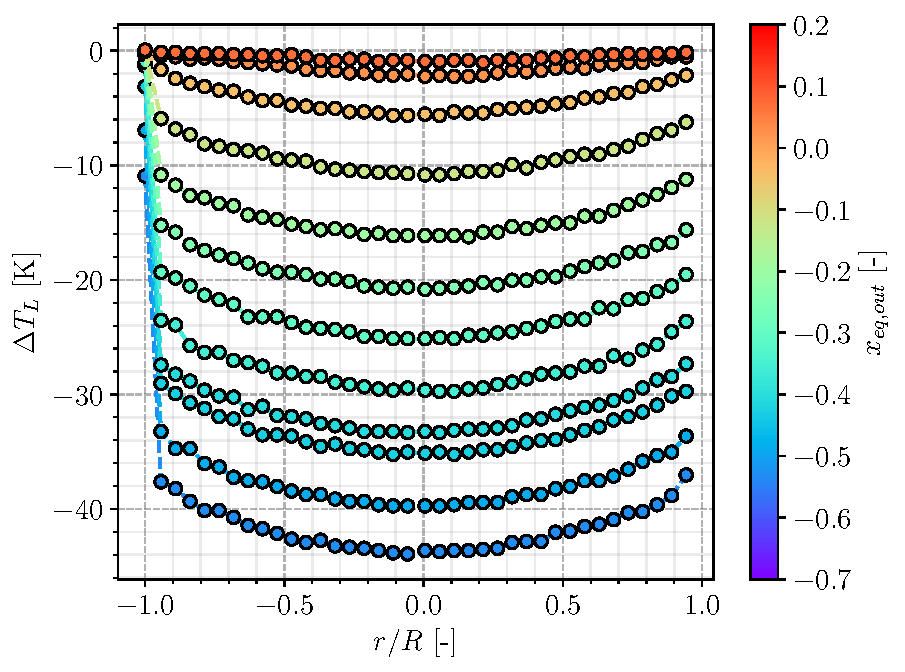
\includegraphics[width=0.5\linewidth]{img/DEBORA/8G2P26W16/8G2P26W16_TL.pdf}
\label{fig:G2P26W16_TL}
}
\subfloat[Liquid subcooling profiles (zoom)]{
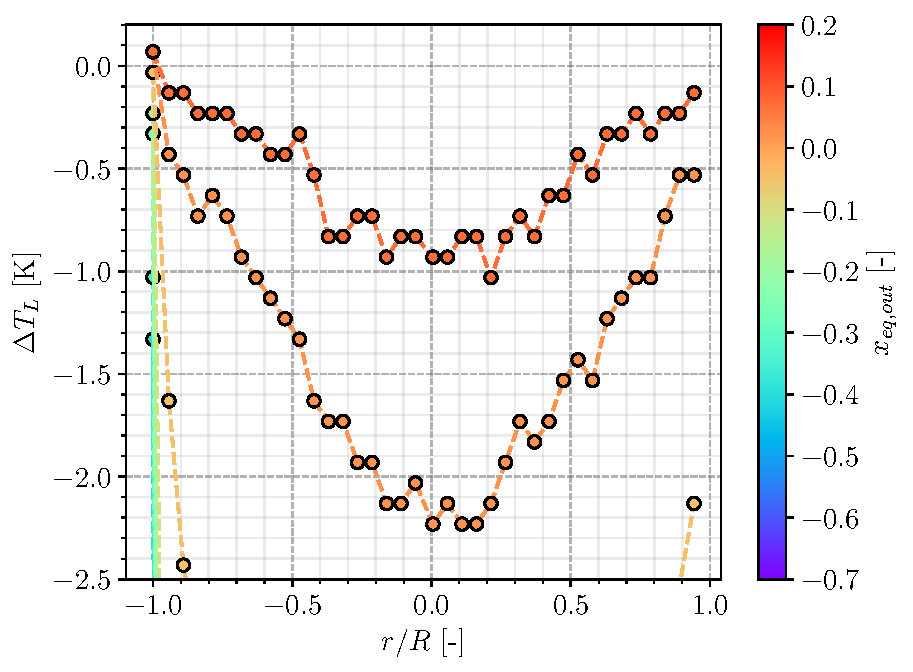
\includegraphics[width=0.5\linewidth]{img/DEBORA/8G2P26W16/8G2P26W16_TLSH.pdf}
\label{fig:G2P26W16_TL_zoom}
}
\\
\subfloat[Wall superheat vs. axial position]{
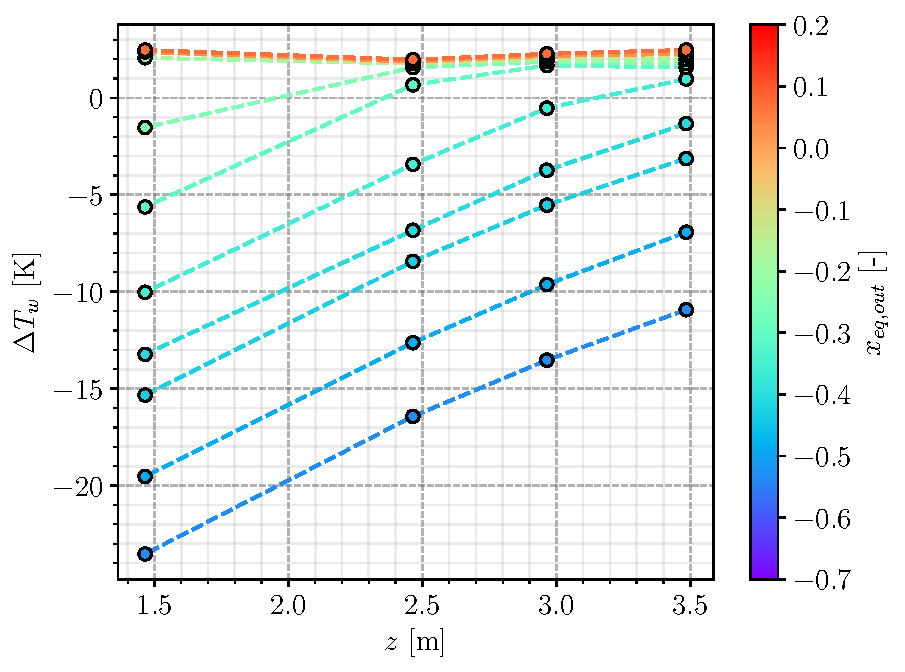
\includegraphics[width=0.5\linewidth]{img/DEBORA/8G2P26W16/8G2P26W16_Tw_z.pdf}
\label{fig:G2P26W16_Twz}
}
\subfloat[Wall superheat vs. local flow quality]{
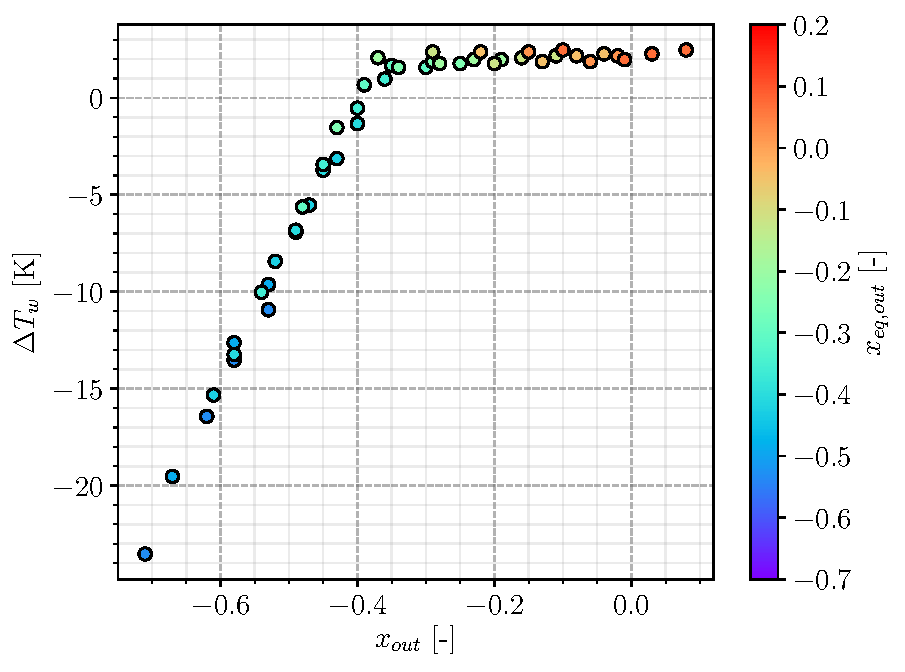
\includegraphics[width=0.5\linewidth]{img/DEBORA/8G2P26W16/8G2P26W16_Tw_x.pdf}
\label{fig:G2P26W16_Twx}
}


\caption{8G2P26W16 results}
\label{fig:8G2P26W16_exp}
\end{figure}

Regarding the liquid temperature measurements (Figures \ref{fig:G2P26W16_TL} and \ref{fig:G2P26W16_TL_zoom}), we see that temperature profiles linearly rise with the inlet quality while presenting an unmodified parabolic shape. The only change appears when reaching significant superheated conditions ($x_{eq,out} \sim 0.1$) where the liquid temperature profile flattens over the test section. 

Moreover, we observe that measurements very close to the wall present a very large temperature gradient even for low quality cases (temperature jump of nearly 30 degrees for coldest cases). This jump reduces as flow quality increases and reduces even more for boiling cases, indicating the well-known rise of the global heat transfer coefficient in boiling regime vs. single-phase convection regime.

We can also note that for the hottest case, the liquid becomes superheated near the wall ($\Delta T_{L}\parth{\pm 1} \approx 0.1\degC$). The bulk is still slightly subcooled with $\Delta T_{L}\parth{0} = -1\degC$

\begin{remark*}{}
The liquid being subcooled in the bulk for superheated cases hints that the decrease in bubble diameter observed in Figure \ref{fig:G2P26W16_dv} for $r/R < 0.6$ may be associated to condensation.
\end{remark*}

\npar

Wall temperature measurements (Figures \ref{fig:G2P26W16_Twz}) display linear growth for subcooled cases which is in agreement with traditional liquid convection problems. When reaching boiling, the wall superheat stabilizes at $\Delta T_{w} \approx 2\degC$.
Rearranging the different wall temperature measurements versus the local flow quality (Figure \ref{fig:G2P26W16_Twx}) presents a coherent overlapping between cases with different inlet subcooling. This further validates the transposition of inlet quality into variation into an evolution of the measurement probe's axial position.


\subsubsection{G2P14W16 cases}


\begin{figure}[h!]
\centering

\subfloat[Void fraction measurements]{
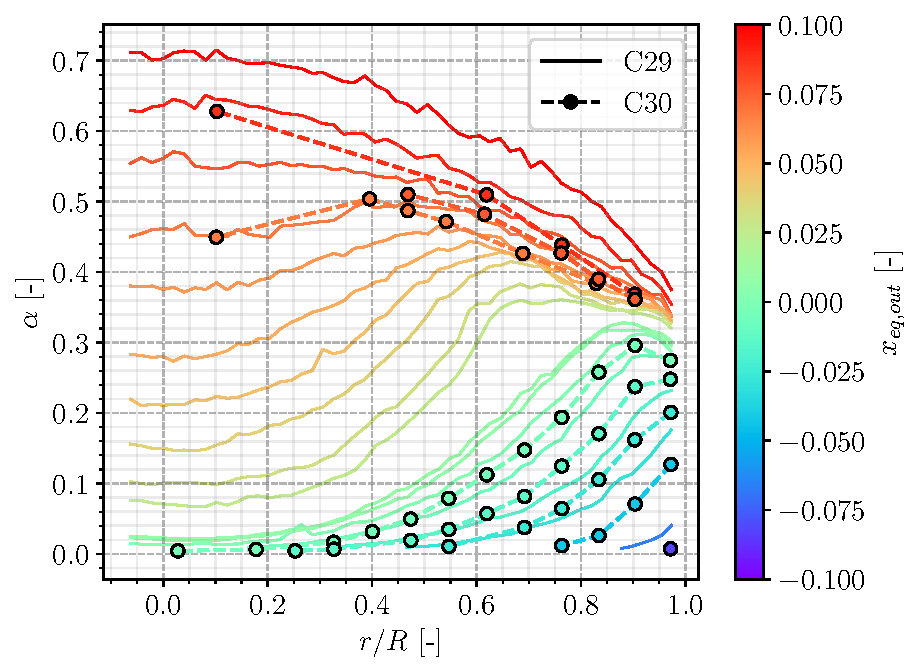
\includegraphics[width=0.5\linewidth]{img/DEBORA/30G2P14W16/30G2P14W16_alpha.pdf}
\label{fig:G2P14W16_alpha}
}
\subfloat[Vapor velocity measurements]{
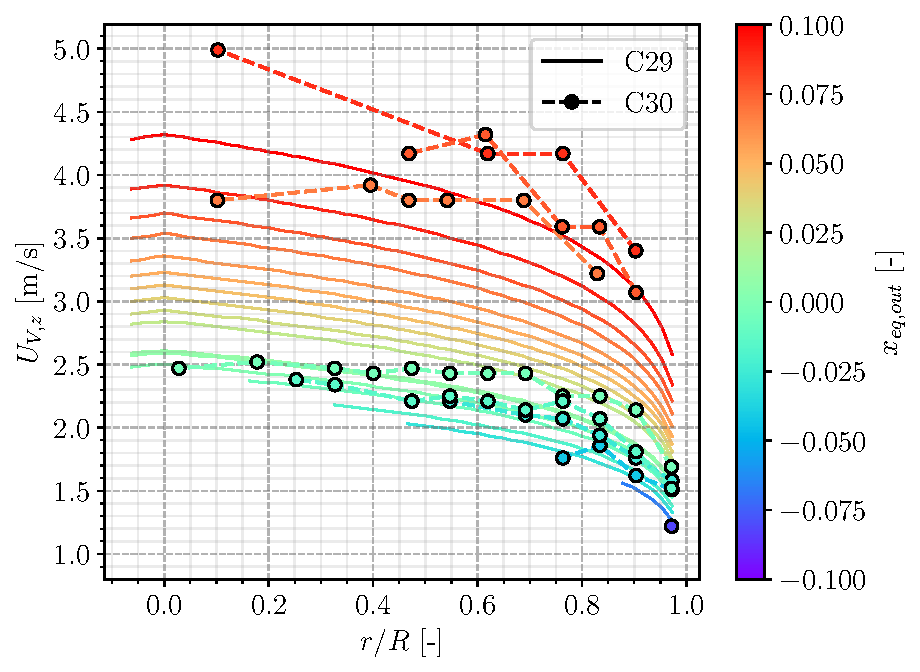
\includegraphics[width=0.5\linewidth]{img/DEBORA/30G2P14W16/30G2P14W16_ugz.pdf}
\label{fig:G2P14W16_ugz}
}
\\
\subfloat[Bubble diameter measurements]{
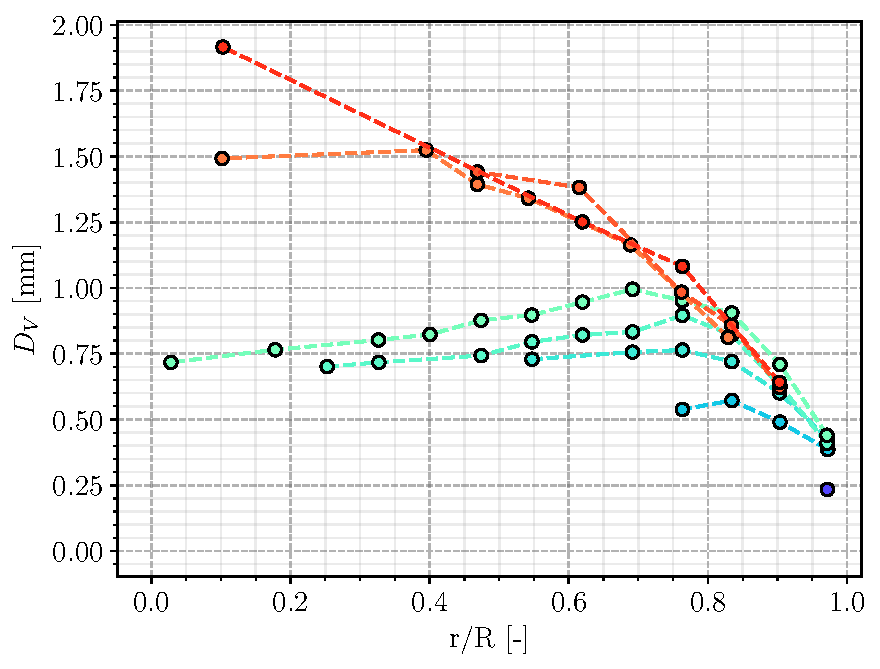
\includegraphics[width=0.5\linewidth]{img/DEBORA/30G2P14W16/30G2P14W16_dv.pdf}
\label{fig:G2P14W16_dv}
}
\subfloat[Interfacial area concentration measurements]{
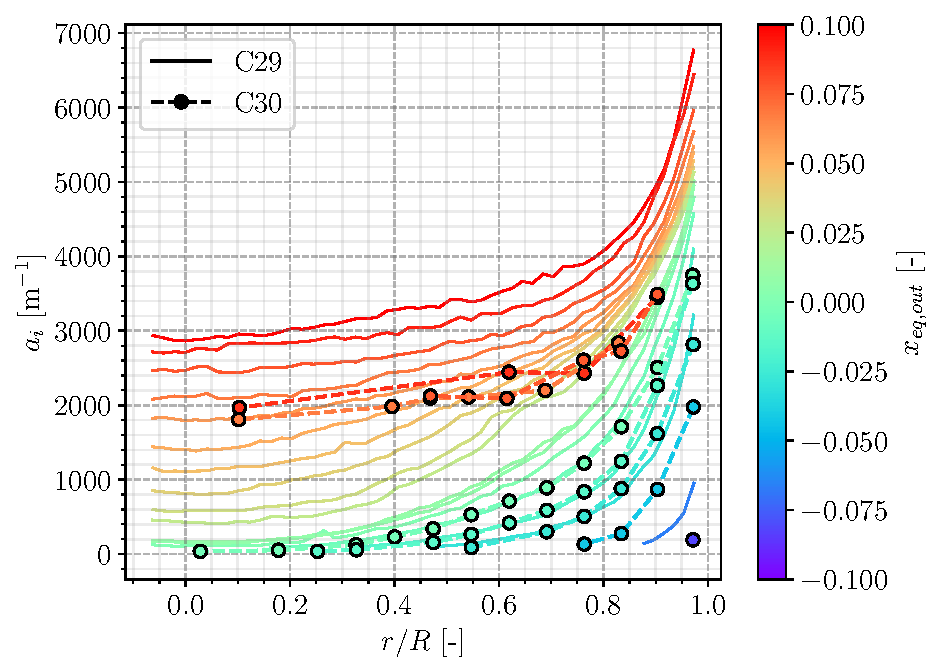
\includegraphics[width=0.5\linewidth]{img/DEBORA/30G2P14W16/30G2P14W16_ai.pdf}
\label{fig:G2P14W16_ai}
}

\caption{30G2P14W16 and 29G2P14W16 results}
\label{fig:30G2P14W16_exp}
\end{figure}



Similar to the G2P26W16 cases, we observe the consistency of the void fraction measurements between the C2900 and C300 campaigns (Figure \ref{fig:G2P14W16_alpha}). Although the vapor velocity estimation using Eq. \ref{eq:ugz_C29} for C2900 cases also produces acceptable results for subcooled cases, the discrepancy when saturation is reached is even more observed here (Figure \ref{fig:G2P14W16_ugz}). The overestimation when $x_{eq,out}>0$ is larger than for the G2P26W16 cases, with nearly 1 m/s error on hottest cases. 

This logically yields larger underestimations of the bubble diameter and associated overestimations of the interfacial area concentration.

\npar

The void fraction profiles (Figure \ref{fig:G2P14W16_alpha}) present a particular evolution with a moving $\alpha$ peak that shifts from the wall to the bulk as the outlet quality increases. This may indicate a particular bubble dynamics regime inducing transverse bubble migration and accumulation far from the wall. Bulk void fraction can reach values as high as 70\% with a flattening profile when $x_{eq,out} \to 0.1$.

\begin{remark*}{}
It seems that saturated cases tend to reach a fixed value of near-wall void fraction between 35\% and 40\%.
\end{remark*}

\npar

Similar to previous obervations, the bubble diameter grows when moving to the bulk, also presenting a peak value around $0.8 > r/R > 0.6$ for subcooled cases (Figure \ref{fig:G2P14W16_dv}). The saturated cases however present much larger increase in bubble diameter when reaching the bulk flow, with $D_{V}$ close to 2 mm for the hottest case. This definitely indicates predominant coalescence effects.

\begin{remark*}{}
$D_{V}\approx 2$ mm is observed at a point where $\alpha >60\%$ which shows that even at such high void fraction values, the flow is still in a bubbly regime with small vapor inclusions ($D_{V} \approx 0.1 D_{h}$).
\end{remark*}

\npar

The vapor velocity also increases with the outlet quality (Figure \ref{fig:G2P14W16_ugz}), but reaches much larger value compared to the G2P26W16 cases. This may be due to the larger bubble size and local void fractions associated to the imposed mass flow rate.


\begin{figure}[h!]
\centering

\subfloat[Liquid subcooling profiles]{
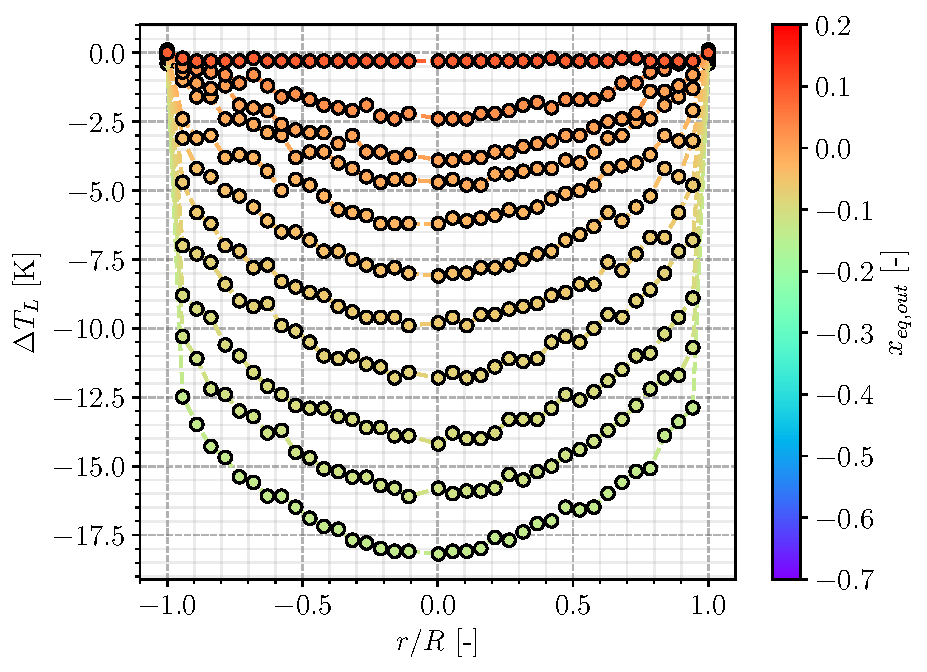
\includegraphics[width=0.5\linewidth]{img/DEBORA/8G2P14W16/8G2P14W16_TL.pdf}
\label{fig:G2P14W16_TL}
}
\subfloat[Liquid subcooling profiles (zoom)]{
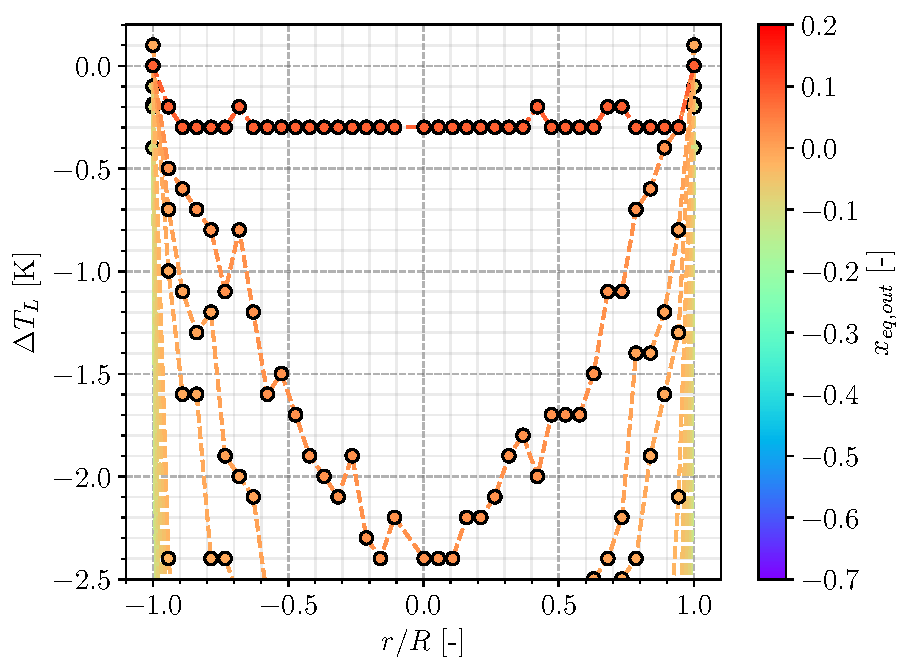
\includegraphics[width=0.5\linewidth]{img/DEBORA/8G2P14W16/8G2P14W16_TLSH.pdf}
\label{fig:G2P14W16_TL_zoom}
}
\\
\subfloat[Wall superheat vs. axial position]{
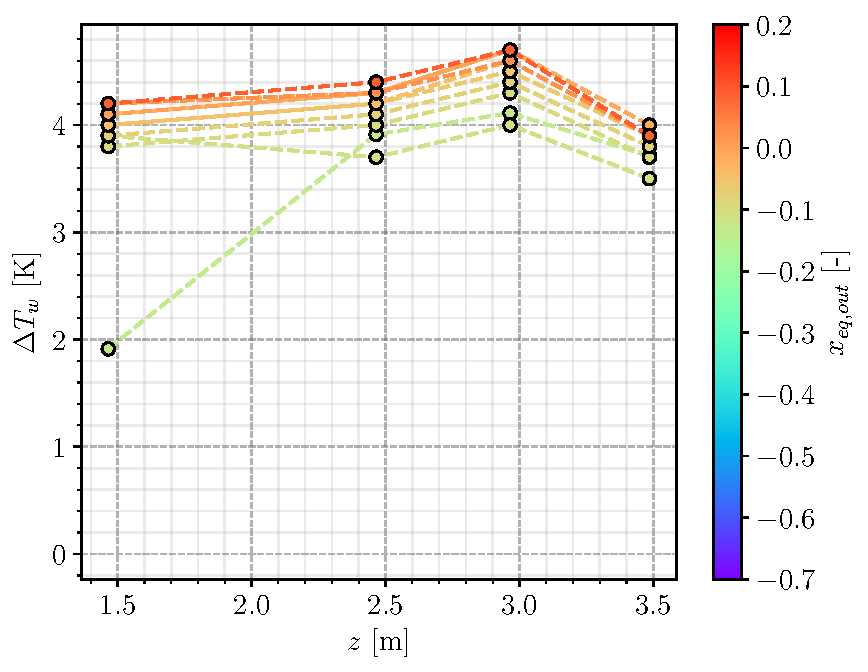
\includegraphics[width=0.5\linewidth]{img/DEBORA/8G2P14W16/8G2P14W16_Tw_z.pdf}
\label{fig:G2P14W16_Twz}
}
\subfloat[Wall superheat vs. local flow quality]{
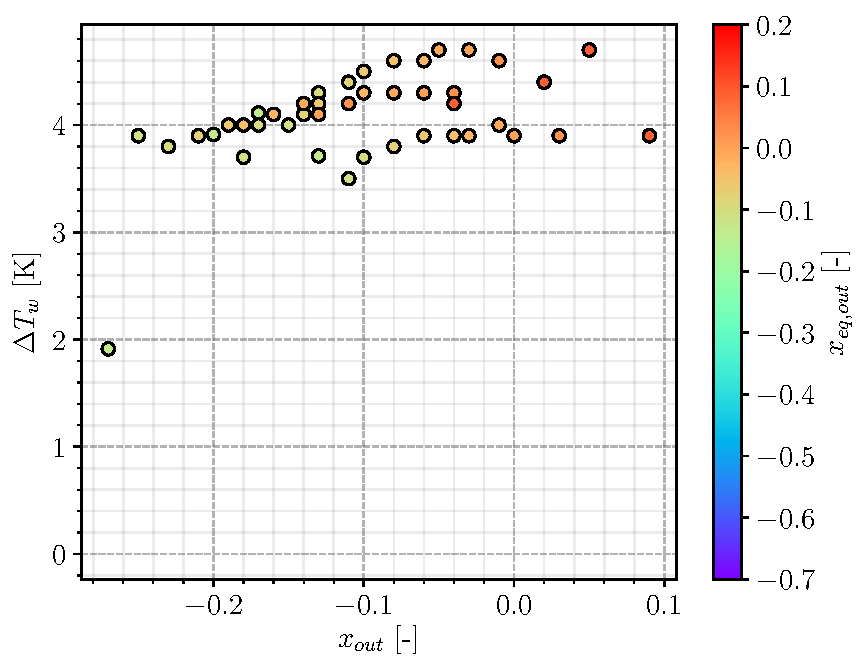
\includegraphics[width=0.5\linewidth]{img/DEBORA/8G2P14W16/8G2P14W16_Tw_x.pdf}
\label{fig:G2P14W16_Twx}
}


\caption{8G2P14W16 results}
\label{fig:8G2P14W16_exp}
\end{figure}


\npar

The liquid temperature profiles (Figure \ref{fig:G2P14W16_TL}) are behaving in a very similar way to the G2P26W16 cases (Figure \ref{fig:G2P26W16_TL}): stable parabolic profile, linear shift with inlet quality and flattening when reaching superheated conditions ($x_{eq,out} \sim 0.1$).

We also have the huge temperature jump when approaching the wall which reduces when reaching boiling regimes. The measurements also detect superheated liquid near the wall for the hottest cases ($\Delta T_{L} \approx 0.1 \degree$). The case with the greatest outlet quality presents a surprisingly flat liquid temperature profile with measurements being nearly constant ($\Delta T_{L}=-0.3\degC$) over the whole measurement section. 

\begin{remark*}{}
Such a constant temperature profile could be interpreted as a limit of the liquid temperature in this regime. Since it corresponds to flow conditions where void fraction is large ($\alpha > 60\%$) and bubbles do not condense (Figure \ref{fig:G2P14W16_dv}), any extra heat input may only contribute to phase change and leave the liquid phase thermally unchanged.
\end{remark*}

\npar

Unfortunately, the 8G2P15W16 campaign did not cover as large quality range as the 8G2P26W16 campaign. We thus do not have access to many single-phase flow wall temperature measurements (Figure \ref{fig:G2P14W16_Twz}). Only one point for $x_{eq,out} \approx -0.1$ seem to be in the single-phase convection region. All the other measurements are close to each other and correspond to boiling regimes where we observe a wall superheat stabilization aroud $\Delta T_{w} = 4\degC$.

The comparison of wall temperature with local flow quality (Figure \ref{fig:G2P14W16_Twx}) is not as interesting as the G2P26W16 cases but still display a welcomed overlapping of the measurements over the different inlet temperatures.


\section{Further Verifications}


\subsection{Reconstruction of the Applied Heat Flux}

To further quantify the coherency of the DEBORA database, we want to reconstruct the wall heat flux injected in the flow from the experimental measurements of void fraction, vapor velocity and liquid temperature measurements.

\subsubsection{Methodology}

To do so, we will estimate the total enthalpy change between the inlet and outlet. The inlet liquid enthalpy $h_{L,in}$ is estimated using the inlet temperature and the outlet mixture enthalpy $h_{M,out}$ is computed as:

\begin{equation}
h_{M,out}=x_{m,out}h_{V,sat}+\parth{1-x_{m,out}}\spavg{h_{L,out}}
\end{equation}
supposing that the vapor is at saturation temperature and where $x_{m,out}$ is the outlet mass quality.

\npar
Using the experimental values of $\alpha$ and $U_{V,z}$, we can compute the outlet mass quality $x_{m,out}$ as:

\begin{equation}
x_{m,out} = \frac{\rho_{V}\spavg{\alpha U_{V,z}}}{G}
\end{equation}

where:

\begin{equation}
\spavg{\alpha U_{V,z}} = \frac{1}{\pi R^{2}}\int_{\vartheta=0}^{2\pi} \int_{r=0}^{R} \alpha\parth{r} U_{V,z}\parth{r} r \mathrm{d}r \mathrm{d}\vartheta = \frac{2}{R^{2}}\int_{r=0}^{R}  \alpha\parth{r} U_{V,z}\parth{r} r \mathrm{d}r
\end{equation}
for an axisymmetric profile such as the DEBORA measurements.

\npar

From the mass quality we can compute the mixture enthalpy as:

\begin{equation}
h_{M} = x_{m} h_{V,sat} + \parth{1-x_{m}} \frac{\spavg{\rho_{L}\parth{1-\alpha}U_{L,z}h_{L}}}{\spavg{\rho_{L}\parth{1-\alpha}U_{L,z}}}
\end{equation}

\npar
Similarly, the average liquid enthalpy at the outlet is estimated as:

\begin{equation}
\spavg{h_{L}} = \frac{2}{R^{2}}\frac{1}{G_{L}}\int_{r=0}^{R} \rho_{L}\parth{r} U_{L,z}\parth{r} h_{L}\parth{r} r \mathrm{d}r
\end{equation}

where $h_{L}$ is estimated using the local temperature measurements and $U_{L,z}$ is estimated using the drift velocity of Ishii \cite{ishii_one-dimensional_1977}:

\begin{equation}
U_{L,z} = U_{V,z} - U_{rel} = U_{V,z} - \sqrt{2} \parth{\frac{g \sigma \parth{\rho_{L}-\rho_{V}}}{\rho_{L}^{2}}}^{1/4} \parth{1-\spavg{\alpha}}^{1.75}
\end{equation}



\npar

Then, writing the one-dimensional energy balance of the flow permits to express the actually applied heat flux: 

\begin{equation}
G \pi R^{2} \parth{h_{M,out} - h_{L,in}} = \Phi_{w} = \phi_{w} 2\pi R L_{heat} \ \Rightarrow \phi_{w} = \frac{\parth{h_{M,out}-h_{L,in}}GR}{2L_{heat}}
\end{equation}
which can be compared to the given control parameter for the experiment.

\subsubsection{Application}

To apply the presented reconstruction of the heat flux, we either need: 

\begin{itemize}
\item A pure single-phase case with an outlet liquid temeprature profile (C800 case alone);
\item A boiling two-phase case with void fraction and vapor velocity measurements (C3000 case) along with liquid temperature (C800 case).
\end{itemize}

This means that for boiling cases, we need to "merge" cases from the C3000 and C800 campaign conducted in very close operating conditions ($P$, $G$, $T_{L,in}$) and assume that the liquid temperature measurements of the C800 case are actually representative of the liquid temperature in the C3000 case and reciprocally for the void fraction and vapor velocity.

\npar

Such a constraint leaves us with very few boiling cases that can accommodate those conditions. They are summed up on Table \ref{tab:debora_match_C8C30}.


\begin{table}[!h]
\centering

\begin{tabular}{c||c|c|c|c|c|c}
Case Name & $P$ [bar] & $G$ [kg/m$^{2}$/s]  & $\phi_{w}$ [kW/m$^{2}$]& $T_{L,in}$ [$\degC$] & $x_{eq,in}$ [-] & $x_{eq,out}$ [-] \\
\hline
\hline
30G2P26W16Te66  &  26.2  &  2049.0  &  73.893  &  66.59  &  -0.2919  &  0.014 \\
8G2P26W16Te66.6  &  26.2  &  1982.0  &  73.9  &  66.57  &  -0.2927  &  0.0237 \\
\hline 
30G2P26W16Te70  &  26.19  &  2051.2  &  73.893  &  70.59  &  -0.2386  &  0.067 \\
8G2P26W16Te70.3  &  26.2  &  1983.0  &  73.9  &  70.31  &  -0.2428  &  0.0734 \\
%\hline
%\hline
%30G2P14W16Te40  &  14.59  &  2007.8  &  77.688  &  41.16  &  -0.1555  &  0.0875 \\
%8G2P14W16Te43.1  &  14.6  &  2014.0  &  72.9  &  43.08  &  -0.1387  &  0.0889 \\
\end{tabular}

\caption{Similar conditions cases between the C3000 and C800 campaigns. Outlet quality calculated with Eq. \ref{eq:xeq_out}.}
\label{tab:debora_match_C8C30}
\end{table}


To actually compute the surface-averaged quantities, we need to interpolate the experimental profiles which is done using the \texttt{python} package \texttt{scipy}. Figure \ref{fig:debora_interpol} presents typical interpolation profiles used in this sections.


\begin{figure}[h!]
\centering

\subfloat[Void fraction interpolation]{
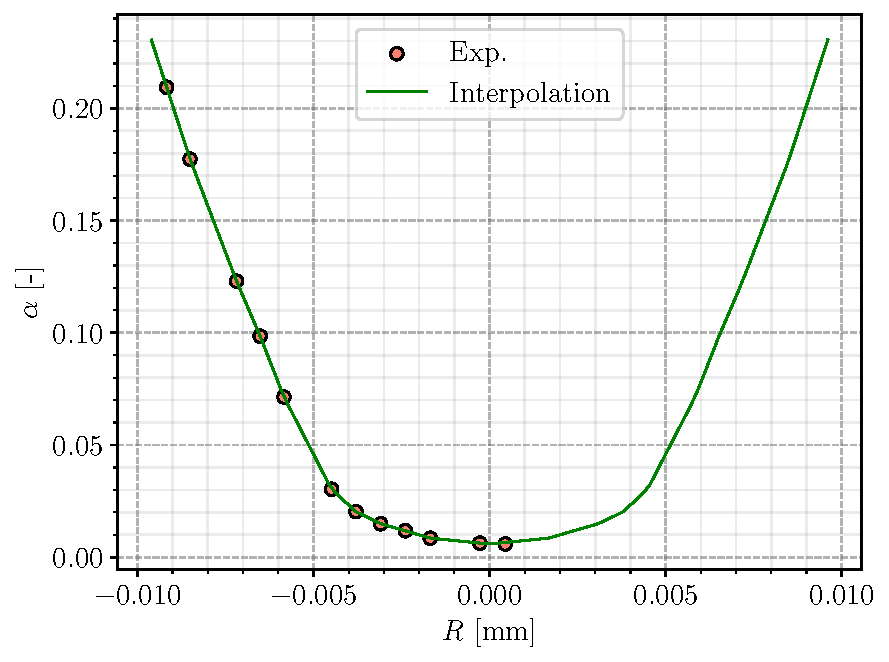
\includegraphics[width=0.4\linewidth]{img/DEBORA/corr_flux/interp_alpha.pdf}
}
\subfloat[Vapor velocity interpolation]{
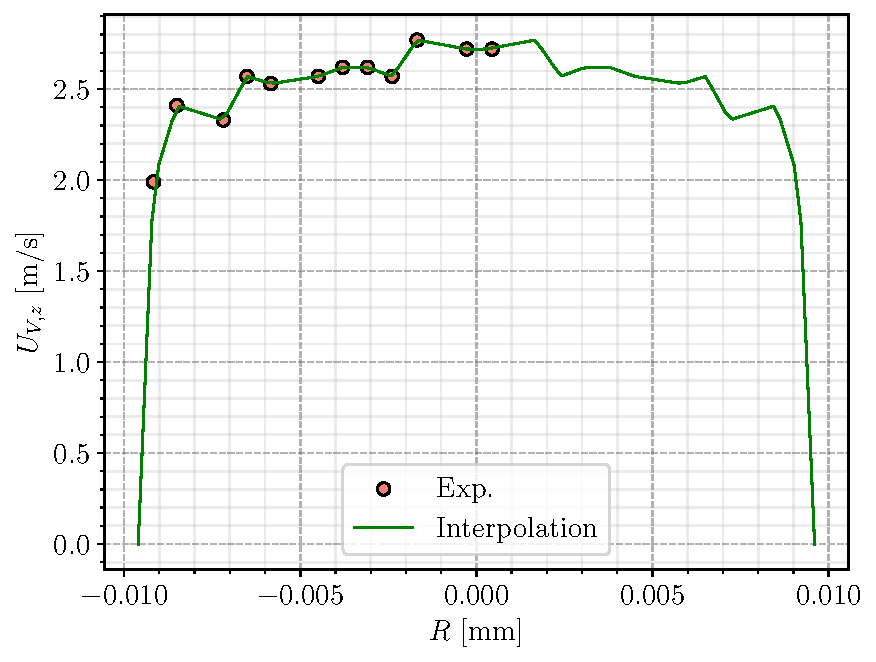
\includegraphics[width=0.4\linewidth]{img/DEBORA/corr_flux/interp_uvz.pdf}
}
\\
\subfloat[Liquid temperature interpolation]{
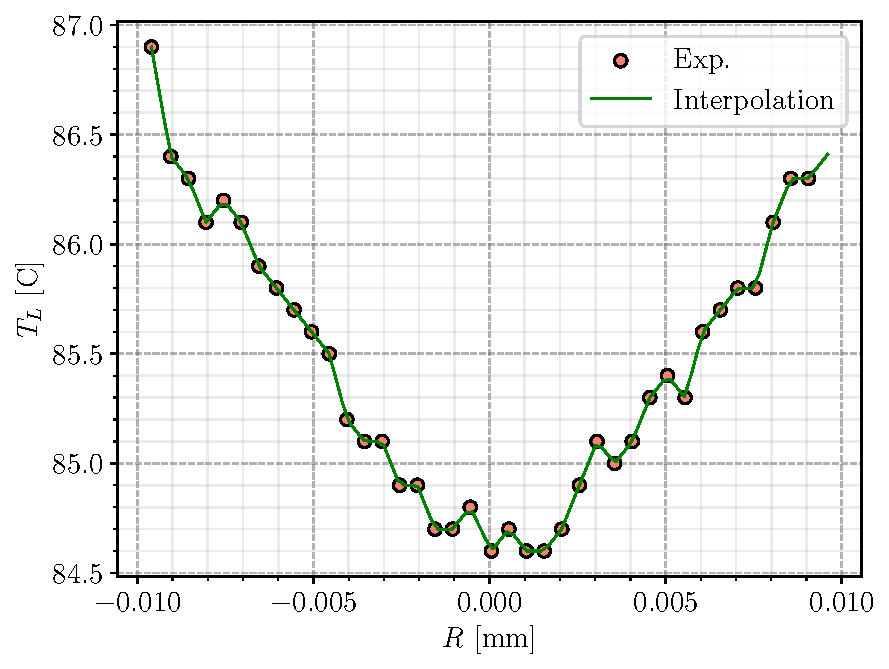
\includegraphics[width=0.4\linewidth]{img/DEBORA/corr_flux/interp_TL.pdf}
}

\caption{Interpolation profiles for cases Te66 (Table \ref{tab:debora_match_C8C30}).}
\label{fig:debora_interpol}
\end{figure}


The results obtained for the heat flux recalculations are presented on Table \ref{tab:debora_flux_corr_res}.

\begin{table}[!h]
\centering

\begin{tabular}{c||c|c|c|c|c}
Case name & $x_{m}$ [-] & $\phi_{w,rec}$ [kW/m$^{2}$] & $\phi_{w,exp}$ [kW/m$^{2}$] & $\Delta \phi_{w}$ [\%]  \\
\hline
\hline
30G2P26W23Te66.6 & 0.0193 & 70.432 & 73.893 & -4.68\%\\
\hline
30G2P26W23Te70.6 & 0.0500\% & 68.041 & 73.893 & -7.9\%\\
%\hline
%\hline
%30G2P14W16Te40 & 0 & 0 & 0 & 0 & 0
\end{tabular}

\caption{Heat flux recalculation results}
\label{tab:debora_flux_corr_res}

\end{table}

We see that reconstructing the heat flux yields values significantly lower than the experimental values given in the database. This underestimation was also noted in a similar approach conducted by Guéguen \cite{gueguen_contribution_2013} who found discrepancy of a few \%.

In our case, these discrepancies can be partially explained by:
\begin{itemize}
\item The difference of inlet mass fluxes that are roughly 70 $\debm$ lower for the C800 cases ;
\item The difference of inlet liquid temperature for the Te70 cases with a C800 case $0.3\degC$ lower than the C300 case.
\end{itemize} 

Those small discrepancies lead to outlet qualities (computed with Eq. \ref{eq:xeq_out} using the given $\phi_{w}$) that differ of approximately $1\%$. Even though boiling flows near saturation, such as those studied here, are very sensitive to the local quality and flow parameters, this would hardly suffice to explain differences in heat flux as much as $5\%$.

\npar
\begin{remark*}{}
Unfortunately, our methodology do not rely on collocated measurements of all the variables of interest since the campaigns were conducted separately. The "correction" values presented in Table \ref{tab:debora_flux_corr_res} can not be considered as accurate estimations but still point out that an uncertainty over the heat flux can be considered in further work.
\end{remark*}



\subsection{Verification of Wall Temperature Measurements}
\label{subsec:debora_Tw_verif}


In order to test the coherency of wall temperature measurements both in single phase and boiling regions, we compare them to one-dimensional correlations along the ($\Delta T_{w}$, $x_{eq}$) curve.

\npar

Single-phase measurements are confronted to the estimations of Dittus-Boelter (Eq. \ref{eq:dittus}) correlation and Gnielinski correlation (Eq. \ref{eq:gnielinski}):

\begin{equation}
\Nu_{DB} = 0.023 \parth{\Re^{4/5}} \Pr^{0.4}
\label{eq:dittus}
\end{equation}

\begin{equation}
\Nu_{G} = \frac{\dfrac{C_{f}}{2} \parth{\Re - 1000} \Pr }{1+12.7\sqrt{\dfrac{C_{f}}{2}} \parth{\Pr^{2/3}-1}}
\label{eq:gnielinski}
\end{equation}
where the friction coefficient $C_{f}$ is estimated following Churchill \cite{churchill_friction_1977} as recommended by Delhaye \cite{delhaye_thermohydraulique_2012} and Guéguen \cite{gueguen_contribution_2013}:

\begin{align}
C_{f} &= 2 \crocht{ \parth{\frac{8}{\Re}}^{12} + \frac{1}{\parth{A+B}^{1.5}} }^{1/12} \\
\nonumber A &=\crocht{ 2.457\ \ln{ \frac{1}{ \parth{\dfrac{7}{\Re}}^{0.9} + 0.27 \dfrac{\varepsilon}{D_{h}} } } }^{16}\ \ \text{($\varepsilon$=0 supposed here)}\\
\nonumber B &= \parth{ \frac{37530}{\Re} }^{16}
\end{align}

\npar

Wall superheat in boiling region is compared with the simple correlation of Frost \& Dzakowic \cite{frost_extension_1967}:

\begin{equation}
\Delta T_{w,FD} = \Pr_{L,sat} \sqrt{\frac{8 \sigma \phi_{w} T_{sat}}{\lambda_{L,sat} h_{LV} \rho_{V}}} 
\label{eq:frost}
\end{equation}
where $T_{sat}$ is expressed in Kelvin.


\npar

The results are presented on Figure \ref{fig:debora_tw_correl_P26} for cases at 26 bar and Figure \ref{fig:debora_tw_correl_P14} for cases at 14 bar. Since we do not need combination with void fraction measurements, every cases of the C800 campaign were used for comparison.


\begin{figure}[h!]
\centering

\subfloat[8G2P14W16 series, $\Delta T_{w,FD}=3.47\degC$]{
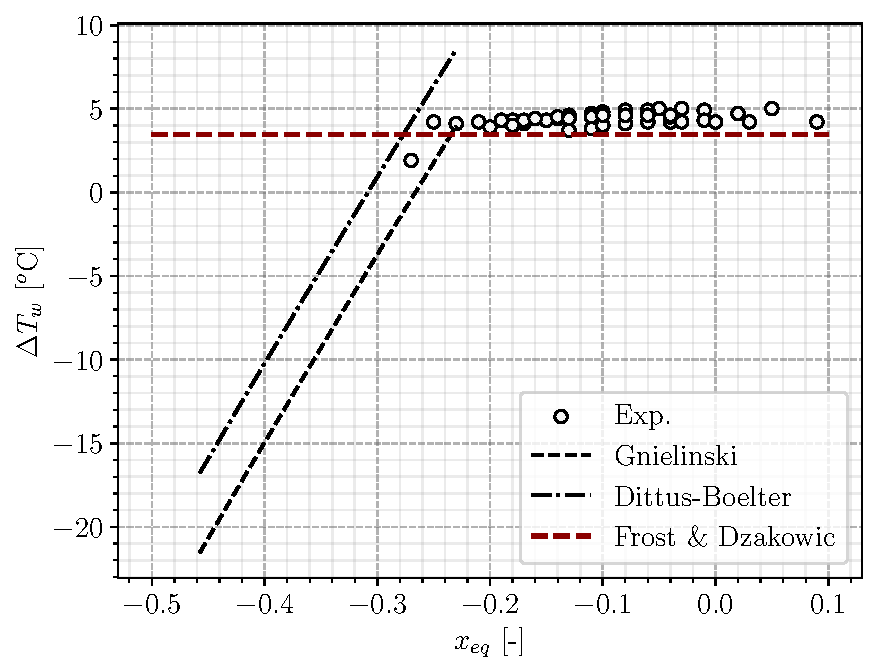
\includegraphics[width=0.5\linewidth]{img/DEBORA/Tw/Tw_8G2P14W16_correl.pdf}
}
\subfloat[8G4P14W24 series, $\Delta T_{w,FD}=4.29\degC$]{
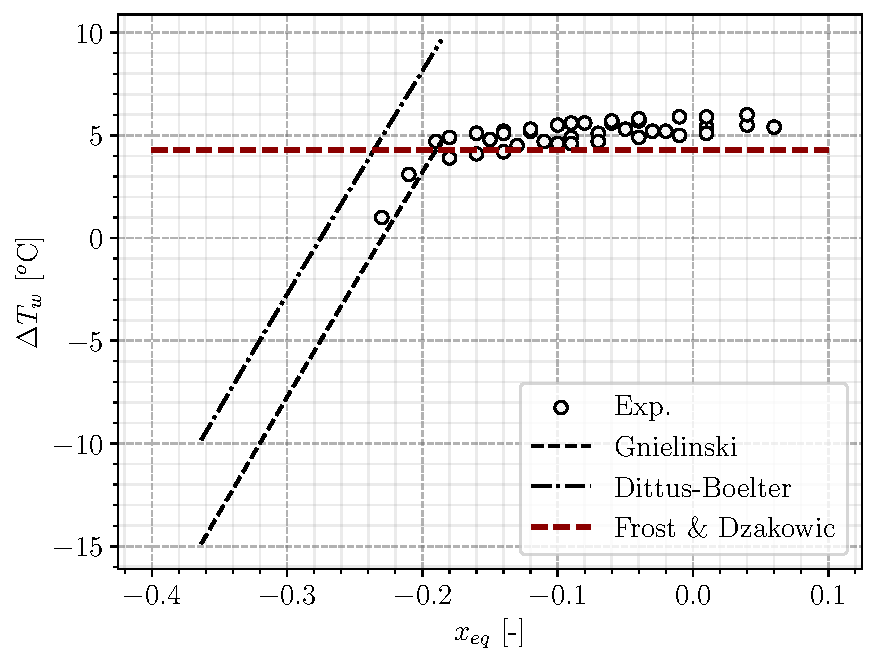
\includegraphics[width=0.5\linewidth]{img/DEBORA/Tw/Tw_8G4P14W24_correl.pdf}
}
\caption{Correlations comparison with P14 cases.}
\label{fig:debora_tw_correl_P14}
\end{figure}


\begin{figure}[h!]
\centering

\subfloat[8G2P26W16 series, $\Delta T_{w,FD}=2.14\degC$]{
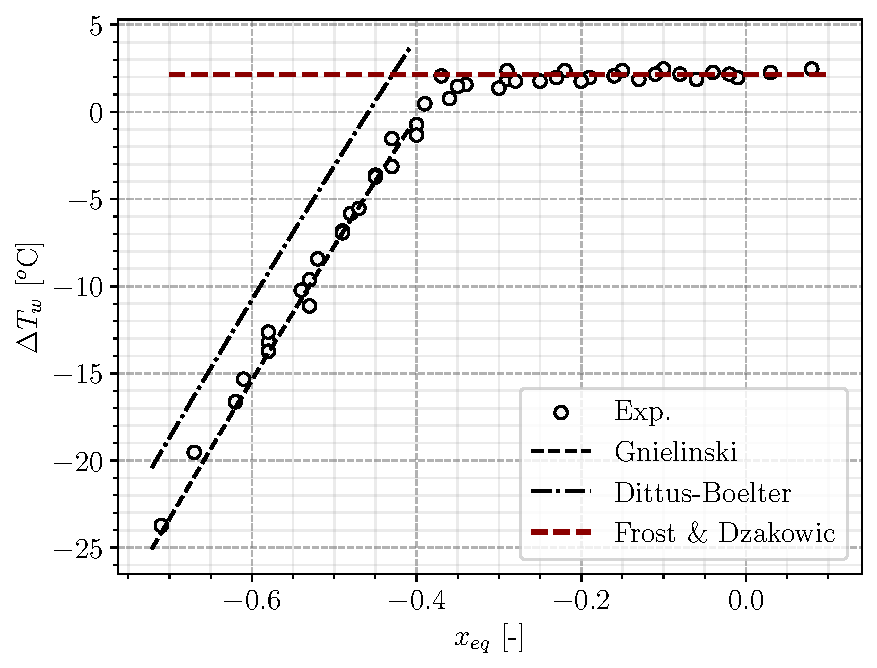
\includegraphics[width=0.5\linewidth]{img/DEBORA/Tw/Tw_8G2P26W16_correl.pdf}
}
\subfloat[8G5P26W16 series, $\Delta T_{w,FD}=2.13\degC$]{
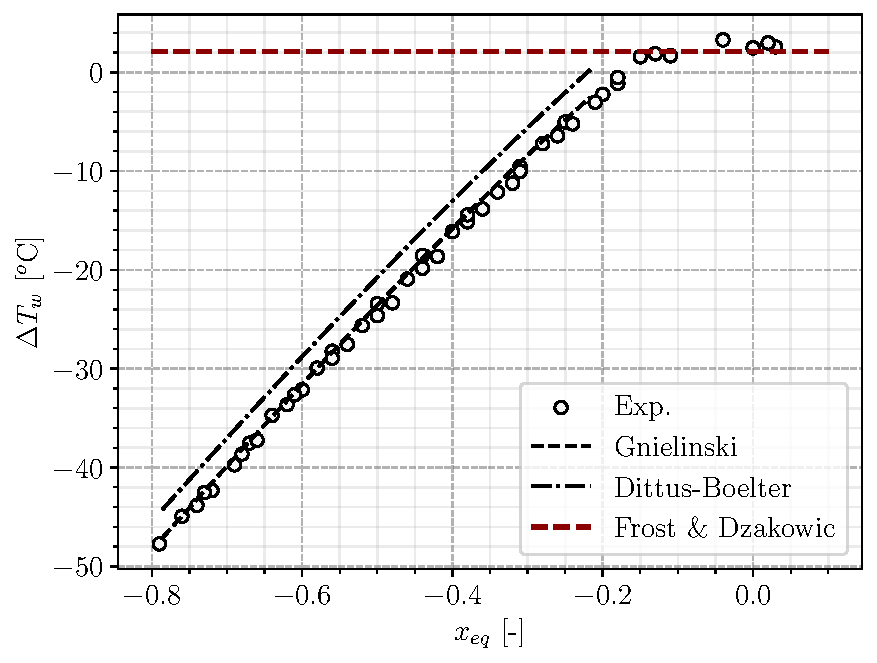
\includegraphics[width=0.5\linewidth]{img/DEBORA/Tw/Tw_8G5P26W16_correl.pdf}
}
\\
\subfloat[8G2P26W24 series, $\Delta T_{w,FD}=2.64\degC$]{
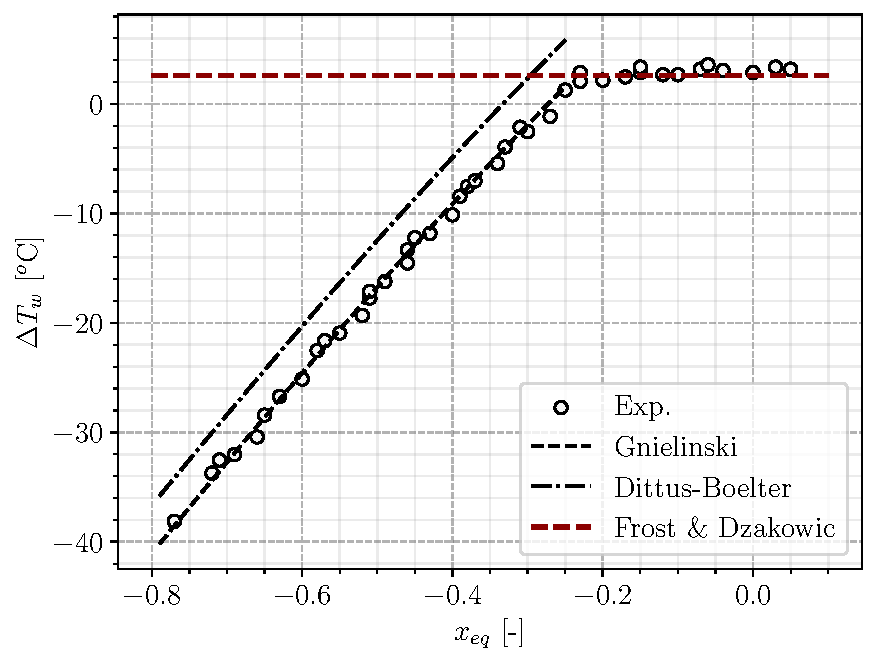
\includegraphics[width=0.5\linewidth]{img/DEBORA/Tw/Tw_8G5P26W24_correl.pdf}
}

\caption{Correlations comparison with P26 cases.}
\label{fig:debora_tw_correl_P26}
\end{figure}


Wall temperature measurements for the liquid convective regime are in fairly good agreement with the predictions of the Gnielinski correlation. The slope of the model is very close to the experimental data in the single-phase region. It is particularly true for the P26 cases (Figure \ref{fig:debora_tw_correl_P26}) where a large range of subcooled conditions in the single-phase region was covered. 

\npar
Regarding the P14 cases (Figure \ref{fig:debora_tw_correl_P14}), very few measurements are available outside of the boiling region. However we can see that the Gnielinski correlation seem to consistently meet the boiling measurements and follow a trend that agrees with the experimental data.

\npar
On the other hand, the Dittus-Boelter correlation fails to predict the wall temperature with a constant overestimation of approximately $5\degC$ regardless of the case. 


\begin{note*}{}
The average liquid temperature at different heights was estimated using a one-dimensional energy balance before computing the local wall temperature predicted by correlations. The virtual length used for single-phase correlations was adjusted to cover the whole range of $x_{eq}$.
\end{note*}

\npar

The nucleate boiling temperature predicted by Frost \& Dzakowic correlation are in good agreement with the exprimental observations where we saw the wall temperature stabilization. The prediction is better for the P26 cases than for the P14 cases where an underestimation of $1\degC$ is observed. We can also note that the measurements are more dispersed for the P14 cases and span over a range of more than $1\degC$ around the average temperature.

\npar

Those comparisons are comforting the consistency of the wall temperature database which correspond to traditional behavior of wall to fluid heat transfer in both single-phase and boiling two-phase regimes.


\section{Conclusions}

The DEBORA database is a very rich source of experimental insights for boiling flows representative of PWR industrial conditions. The large range of control parameters that was covered during the tests also is encouraging regarding the variety of flow regimes that can occur in PWR conditions

\npar

After a finer analysis of the data, in the continuation of the work of Cubizolles \cite{cubizolles_etude_1996}, Manon \cite{manon_contribution_2000} and Guéguen \cite{gueguen_contribution_2013}, we concluded that:

\begin{itemize}
\item The test matrix unfortunately shows that very few series were covered with both bi-optical probe (C3000) and thermocouples (C800) measurements, limiting the availability of a full boiling database to the series G2P26W16 and G2P14W16.

\item Small but significant errors on the reported outlet quality could be observed when compared to a one-dimensional energy balance based on the control parameters (Table \ref{tab:xout_30P26_recalc}).

\item Good agreement was found between the void fraction measurements with the mono (C2900) and bi-optical probe (C3000), which comforts the validity of the acquired data in close flow conditions.

\item Extension of the C2900 data to estimate bubble diameter and interfacial area concentration using Eq. \ref{eq:ugz_C29} to compute vapor velocity was acceptable in subcooled conditions but showed increasing underestimations in the saturated region (Figures \ref{fig:G2P26W16_ugz} and \ref{fig:G2P14W16_ugz}).

\item Void fraction measurements in the G2P14W16 series showed a particular behavior with a peak value moving from the wall to the bulk as the inlet temperature increases.

\item Bubble diameter measurements clearly exhibited coalescence phenomena when leaving the wall with a maximum value reached at $r/R \approx 0.6$ before decreasing under condensation and / or break-up (Figure \ref{fig:G2P26W16_dv}). It was also observed that measurements closest to the wall were nearly constant among a given test series regardless of the inlet temperature.

\item Liquid temperature can overcome the saturation temperature for the hottest cases close to the wall ($T_{L}-T_{sat}\approx 0.1\degC$) and flattens at the bulk with a subcooling roughly around $0.5\degC$.

\item Wall temperature measurements followed a coherent linear profile in the single-phase region before stabilizing when boiling starts, which was further reproduced by comparison with one-dimensional correlations. Measurements were also overlapping each other when plotted versus the local quality, confirming the transposition between change of inlet temperature and axial translation of the measurement section.

\item Reconstruction of the applied wall heat flux in the experiments by merging the values from very close C3000 and C800 cases (Table \ref{tab:debora_match_C8C30}) suggested that the heat flux values provided in the measurements were too large by $5\%$ to $8\%$. Such a large difference is surprising and could partially be explained by the small change of operating conditions between C3000 and C800 cases.
\end{itemize}


At last, the different evaluations conducted over the chosen experiments have reasonably validated the consistency and coherency of the measurements. Further comparisons with NEPTUNE\_CFD simulations will be conducted using the experimental results of the G2P26W16 series. \textbf{ Still, we keep in mind that an error of a few $\%$ is possible on $\phi_{w}$.}




\chapter{NEPTUNE\_CFD simulations of DEBORA cases}
\label{chap:ncfd}

In this work, we present the simulations of the following cases:
\begin{itemize}
\item C8G2P26W16Te44.9 and C8G2P26W16Te49.6 (single-phase flow)
\item C8G2P26W16Te66.6 and C8G2P26W16Te70.3 (two-phase flow)
\item C30G2P26W16Te66.6 and C30G2P26W16Te70.6 (two-phase flow)
\end{itemize}

The pressure of $26~\text{bar}$ is chosen to match the pressure of the mixing vanes cases (DEBORA-Promoteur, Section \ref{sec:deb_prom}). Mesh sensitivity is performed over two meshes: a large mesh (M1) with $460~356\text{ cells }=338\text{ radial } \times 1362 \text{ axial cells}$ and a fine mesh (M2) with $3~157~952\text{ cells }=1568\text{ radial } \times 2014 \text{ axial cells}$.

On Figure \ref{fig:th_1phi_res}, we present the results regarding liquid temperature at the outlet and wall temperature. The liquid temperature profile seems to be correctly reproduced by the simulations, though we see a slight overestimation close to the wall. Looking closer at boiling cases shows a difference of $\approx 0.5\degree$ C, which is close to the uncertainty of the measurements \cite{garnier_local_2001}. Concerning the wall temperature, it appears that it is underestimated before the \textbf{Onset of Nucleate Boiling} (ONB) ($T_{w}<T_{sat}$) and overestimated after the ONB ($\approx +5\degree$C). Post-ONB wall temperature is characterized by a stabilization of its value above the saturation temperature (here $T_{w,ONB}-T_{sat}\approx 2\degree\text{C}$).

%
\begin{figure}[h!]
\centering
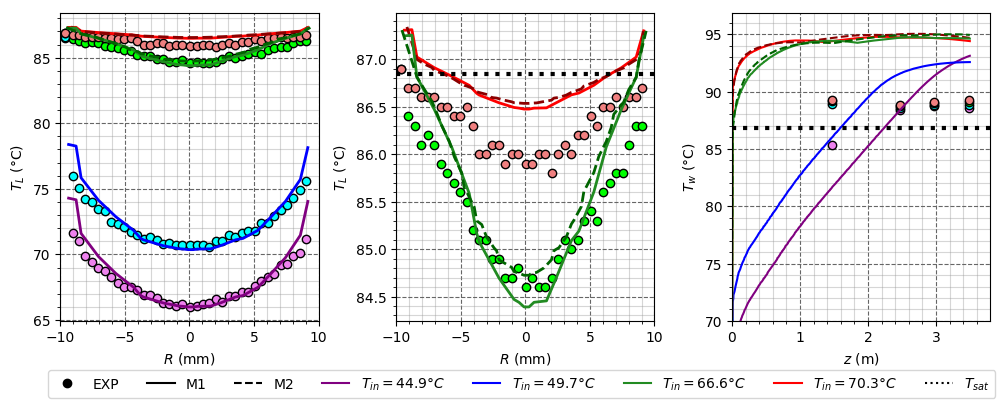
\includegraphics[scale=0.60]{img/DEBORA/c8.png}
\caption{NCFD (lines) vs. Exp. (circles) - $T_{L}$ and $T_{w}$ - Cases C8G2P26W16Te44.9, Te49.6, Te66.6 and Te70.3 - Simulations using two meshes M1 (coarse) and M2 (fine).}
\label{fig:th_1phi_res}
\end{figure}
%

%%
%\begin{figure}[!htb]
%\vspace{16pt}
%\begin{spacing}{1.0}
%\centering
%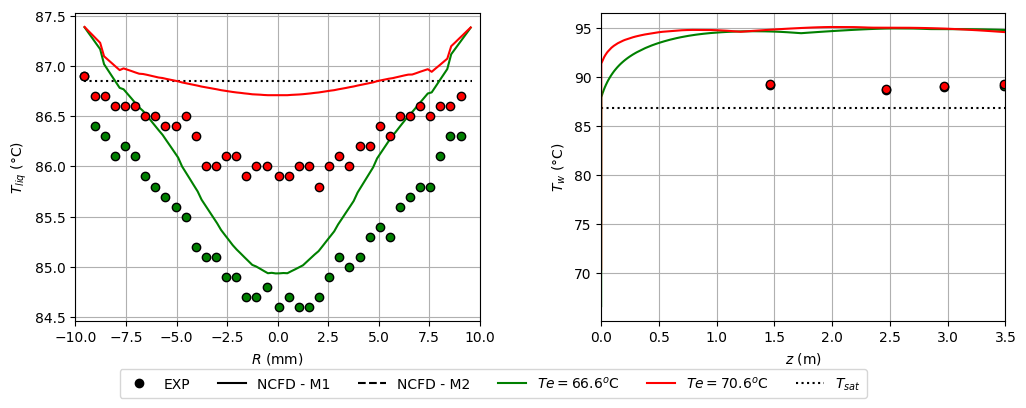
\includegraphics[scale=0.60]{img/DEBORA/thermal_diph.png}
%\caption{NEPTUNE\_CFD simulations results vs. experimental measurements - $T_{L}$ and $T_{w}$ - Cases C8G2P26W16Te66.6 and C8G2P26W16Te70.3}
%\label{fig:th_diph_res}
%\end{spacing}
%\vspace{16pt}
%\end{figure}
%%



%
\begin{figure}[h!]
\centering
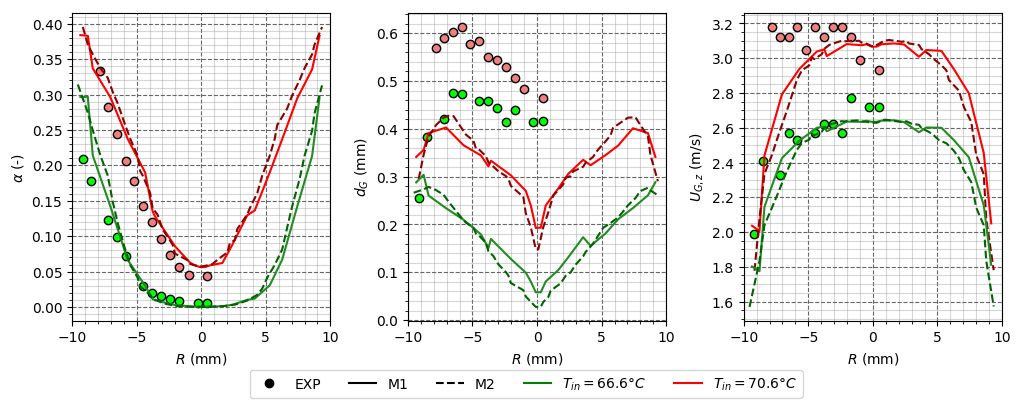
\includegraphics[scale=0.60]{img/DEBORA/c30.png}
\caption{NCFD (lines) vs. Exp. (circles) - $\alpha$, $d_{G}$ and $U_{G,z}$ - Cases C30G2P26W16Te66.6 and Te70.6 - Simulations using two meshes M1 (coarse) and M2 (fine).}
\label{fig:topology_res}
\end{figure}
%

On Figure \ref{fig:topology_res}, we compare the results of the simulations to the experiments regarding void fraction, bubble Sauter diameter and axial gas velocity. Void fraction profiles are quite correctly reproduced, though we observe a $10\%$ higher peak at the wall for $T_{in}=66.6\degree$C. The order of magnitude of bubble diameter is correct ($\sim 0.1\text{mm}$) and NEPTUNE\_CFD manages to detect coalescence (increase of bubble diameter when leaving the wall) and bulk condensation (decrease of bubble diameter when reaching the core of the flow), which is in qualitative agreement with the experiments. Quantitatively speaking, bubble diameter is globally underestimated. Finally, gas velocity profile is reasonably reproduced for $T_{in}=66.6\degree$C, but not for $T_{in}=70.6\degree$C. The latter experimental profile is flatter, which could be explained by a change of flow regime since uncondensed vapor is detected in the bulk.  

Finally, the simulations reasonably agree with the experiments. The strongest discrepancies being mostly the wall temperature and bubble diameter. Potential ways of improving those results are investigated in next sub-section.

\subsection{Investigating the nucleation site density modeling $N_{sit}$}

In NEPTUNE\_CFD, wall temperature is computed through the Heat Flux Partitioning model, which role is to find the appropriate $T_{w}$ which balances Equation $\ref{eq:HFP}$. However, some laws used to express parameters such as $N_{sit}$, $f$, or $d_{d}$ are quite old and simple. For instance, the {Lemmert} \& {Chawla}\cite{lemmert_influence_1977} expression of $N_{sit}$ only depends on the wall superheat (Sub-section \ref{subsec:HFP}).%, meaning that it can not reproduce potential influence of the pressure on the nucleation site density.

A comparison of the {Lemmert} \& {Chawla} law\cite{lemmert_influence_1977} with  the {Hibiki} \& {Ishii}\cite{hibiki_active_2003} law for $N_{sit}$ against 4 data sets from the literature is presentend on Figure \ref{fig:nsit}. The {Hibiki} \& {Ishii} correlation depends simultaneously on wall superheat, pressure and contact angle.  Experimental measurements of {Borishanskii} \etal\cite{borishanskii_heat_1969}, {Richenderfer} \etal\cite{richenderfer_investigation_2018}, {Kossolapov} \etal\cite{kossolapov_experimental_2021} and {Zhou} \etal\cite{zhou_experimental_2020-1} are used to assess the two nucleation site density correlations.
%
\begin{figure}[h!]
\centering
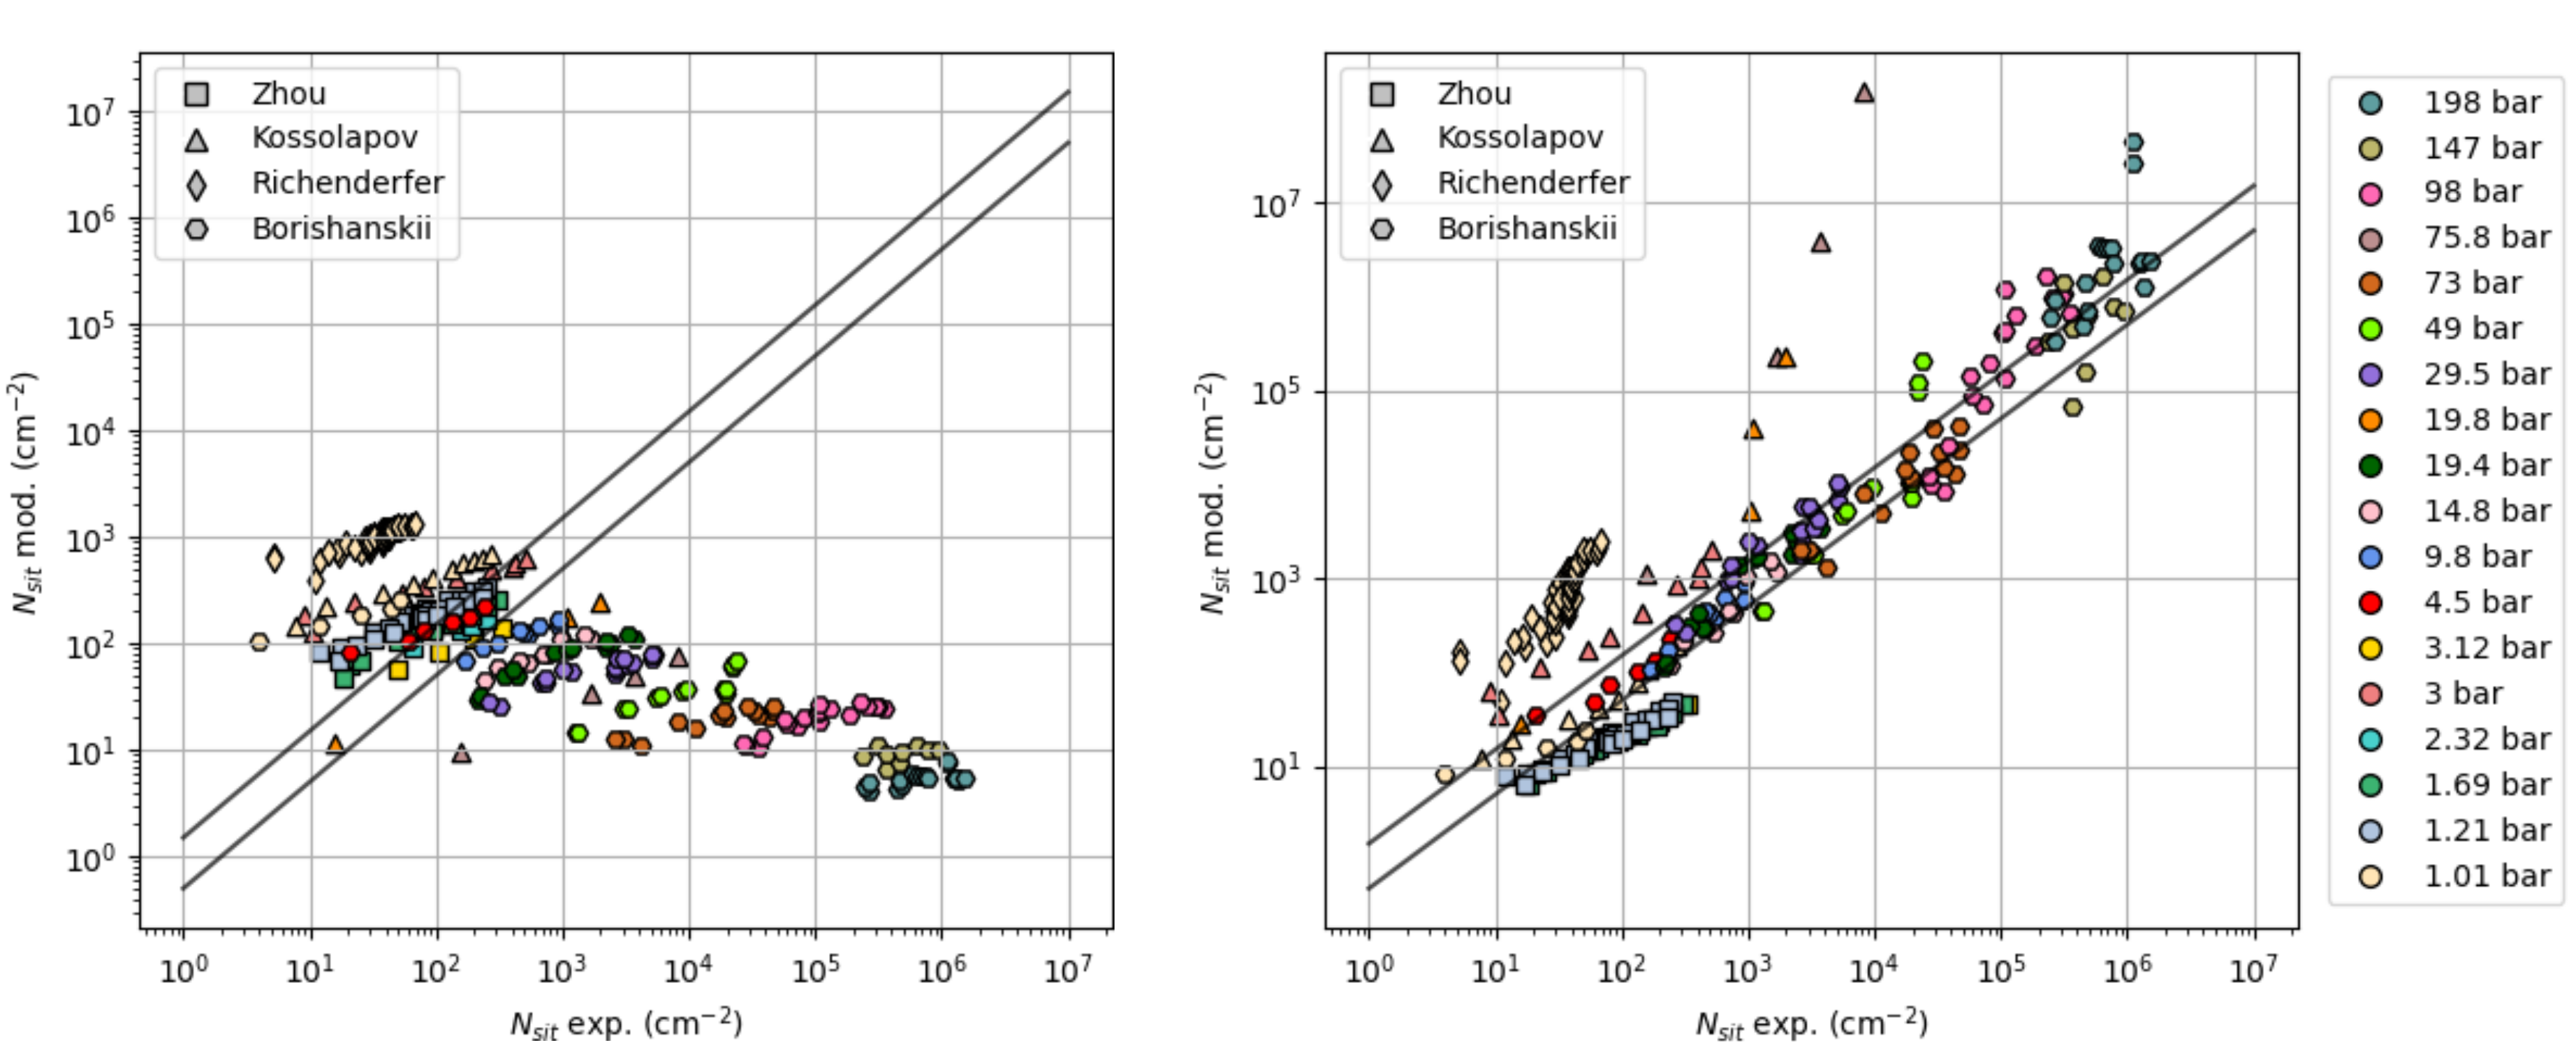
\includegraphics[scale=0.45]{img/DEBORA/nsit.png}
\caption{$N_{sit}$ correlations of {Lemmert} \& {Chawla} (left) and {Hibiki} \& {Ishii} (right) vs. exp. data from literature. Operation pressures are displayed. $\pm 50\%$ error bars are drawn in black.}
\label{fig:nsit}
\end{figure}
%

Figure \ref{fig:nsit} clearly shows that the {Lemmert} \& {Chawla} law lack of pressure dependence fails to reproduce high pressure measurements contrary to the {Hibiki} \& {Ishii} one. Even though {Hibiki} \& {Ishii} correlation shows significant discrepancies with measurements of {Kossolapov} \etal and {Richenderfer} \etal, its prediction capability is greater in average than {Lemmert} \& {Chawla} correlation.

%
\begin{figure}[h!]
\centering
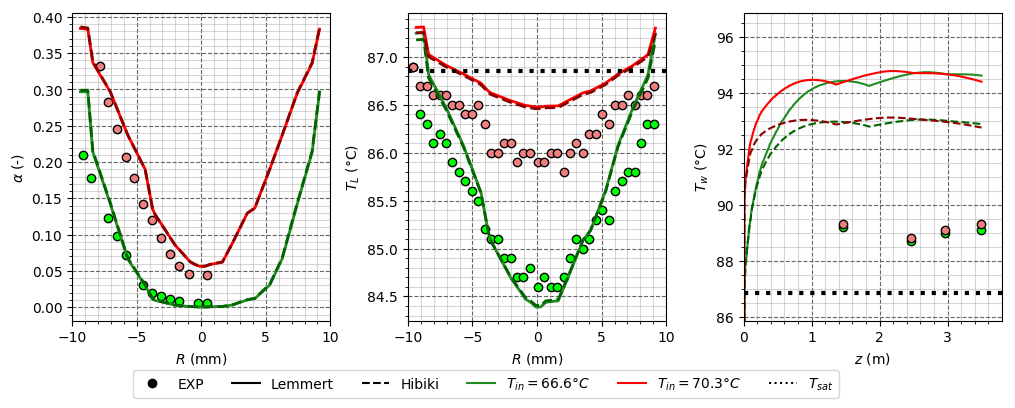
\includegraphics[scale=0.60]{img/DEBORA/plot_HI.png}
\caption{NCFD results for $\alpha$, $T_{L}$ and $T_{w}$ using {Lemmert} \& {Chawla} and {Hibiki} \& {Ishii} correlation. Cases 8G2P26W23Te66.6 and Te70.3, 30G2P26W23Te66.6 and 70.6.}
\label{fig:NCFD_nsit}
\end{figure}
%
To assess the influence of nucleation site density law on NEPTUNE\_CFD computations, we compare results obtained with both correlations on Figure \ref{fig:NCFD_nsit}, which shows a remarkable impact of the modification of $N_{sit}$ correlation. Using {Hibiki} \& {Ishii} correlation reduces the error on $T_{w}$ by approximately $2\degree\text{C}$ while $\alpha$ and $T_{L}$ remain unchanged. This implies that the same heat flux partitioning is found with the two models, but that the pressure dependence of {Hibiki} \& {Ishii} law helped to balance Equation \ref{eq:HFP} using a lower $T_{w}$, thus closer to experimental measurements.

Such a result indicates that the HFP model could be improved through a systematic analysis of each parameter's impact and modeling (bubble departure diameter, detachment frequency, etc.). Assembling a more recent and consistent model could provide better results regarding wall temperature prediction. Models such as the one developed by {Kommajosyula}\cite{kommajosyula_development_2020} could be interesting to apply for high-pressure flows.


Now that simple tube boiling flow has been assessed through the presented results, next section will focus on the simulation of boiling flow in a tube equipped with a mixing device.% using DEBORA-Promoteur experimental results.